\documentclass{article}


\usepackage{arxiv}

\usepackage[utf8]{inputenc} % allow utf-8 input
\usepackage[T1]{fontenc}    % use 8-bit T1 fonts
\usepackage{hyperref}       % hyperlinks
\usepackage{url}            % simple URL typesetting
\usepackage{booktabs}       % professional-quality tables
\usepackage{amsfonts}       % blackboard math symbols
\usepackage{nicefrac}       % compact symbols for 1/2, etc.
\usepackage{microtype}      % microtypography
\usepackage{lipsum}
\usepackage{graphicx}
\usepackage{amsmath}
\usepackage{verbatim}
\usepackage{caption}
\usepackage{subcaption}

\usepackage{float}
\restylefloat{table}


\title{Evaluation on accuracy of mapping science to the United Nations' Sustainable Development Goals (SDGs) of the Aurora SDG queries}


\author{
  Felix Schmidt \\
  University Library\\
  University of Duisburg-Essen\\
  Duisburg, Germany\\
  \texttt{felix.schmidt@uni-due.de} \\
  %% examples of more authors
   \And
Maurice Vanderfeesten \\
  University Library\\
  Vrije Universiteit Amsterdam\\
  Amsterdam, The Netherlands \\
  \texttt{maurice.vanderfeesten@vu.nl} \\
  %% \AND
  %% Coauthor \\
  %% Affiliation \\
  %% Address \\
  %% \texttt{email} \\
  %% \And
  %% Coauthor \\
  %% Affiliation \\
  %% Address \\
  %% \texttt{email} \\
  %% \And
  %% Coauthor \\
  %% Affiliation \\
  %% Address \\
  %% \texttt{email} \\
}

\begin{document}
\maketitle

\begin{abstract}
In this study we evaluate the accuracy of our Aurora SDG classification model version 5, to match research papers to the Sustainable Development Goals (SDG's) of the United Nations. The aim of this investigation is to be transparent about the accuracy of the model, because this model might get used in reporting and strategy analysis by University leadership. The measurements are based on a baseline, 'golden set', where researchers of the Aurora universities handpicked publications that relate to an SDG. We measured the Precision and Recall of the Aurora model, and relating it to our previous version of the model, and to the Elsevier SDG model. 
\end{abstract}


% keywords can be removed
\keywords{Bibliometrics \and SDG's \and  Sustainable Development Goals \and  Precision \and Recall \and Scientific publications \and Mapping \and Boolean search queries \and Scopus}


\section{Introduction}
The Aurora is a network of nine leading European research universities founded in 2016, united by their commitment to match academic excellence with creating societal impact. University leadership asked to demonstrate the relevance of their research to grand societal challenges \cite{drooge_evaluating_2010} \cite{carley_social_2019}. Therefore the Sustainable development goals (SDG's) of the United Nations were chosen as a framework to be the leading narrative, to match research papers to these topics using boolean search queries \cite{armitage_mapping_2020}. The bibliometricians of the Aurora universites have worked together since 2017 for create our own definition of the \emph{"Aurora SDG Queries"} to match our research to the SDG's. Since the start of the Aurora SDG Matching Initiative \footnote{\url{https://aurora-network.global/project/sdg-analysis-bibliometrics-relevance/}}, many other initiatives got inspired and started as well, such as the \emph{"Elsevier SDG Queries"} \cite{jayabalasingham_identifying_2019}  in 2019 focused on recall for the Times Higher Impact Ranking. Aurora has their own set of SDG queries with a focus on precision rather then recall. Also the \emph{"Aurora SDG Queries"} has the capability to find literature on the narrower level of the targets, next to the broader level of the Goals. This allows us to identify researchers within the university network who work on research related to similar societal challenges of the narrower target level.  With these SDG labeled research papers the data was enriched to provide information on the academic excellence and societal impact \cite{bornmann_what_2013} using citation and altmetric databases, but that is out of scope for this report. 

\begin{figure}[ht]
	\centering
  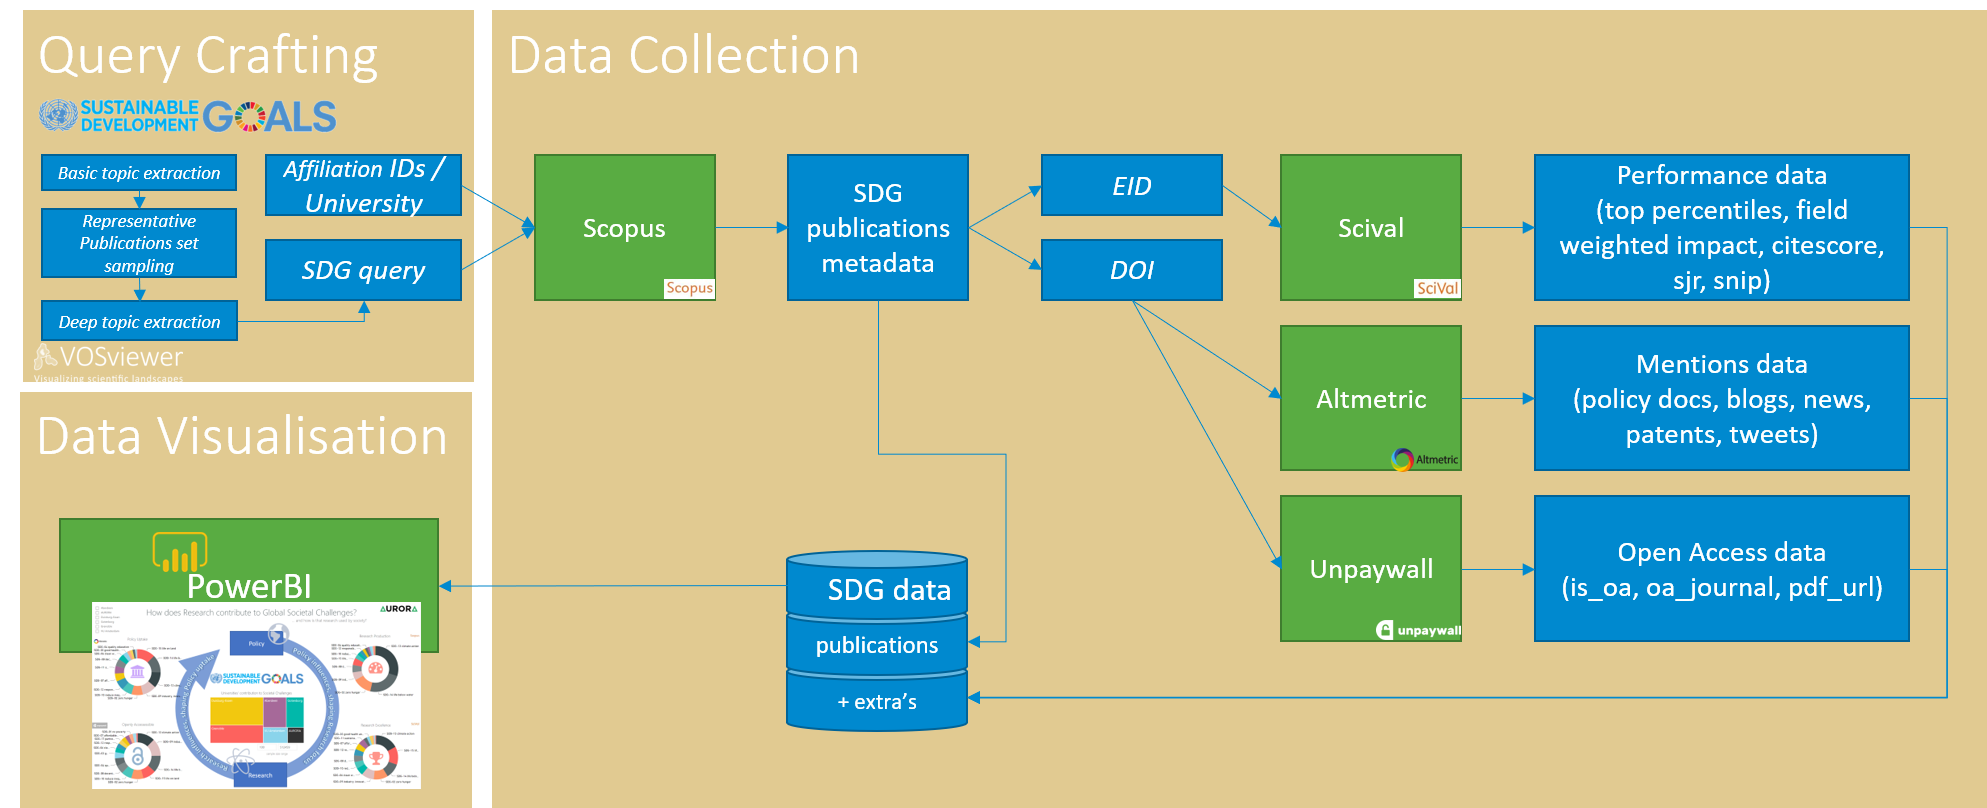
\includegraphics[width=0.9\textwidth]{figures/sdg-data-workflow.png}
	\caption{Workflow collecting data.}
	\label{sdgdataworkflow}
\end{figure}

We have created the initial version of the \emph{"Aurora SDG Queries"} by simply using the significant keywords in the policy texts of the Sustainable Development Goals, Targets and Indicators \footnote{\url{http://metadata.un.org/sdg/}}, using boolean search operation structure in such way (combining groups of concepts, synonyms and antonyms with near-operators), that the search results minimize false positives. We incrementally improved the queries, and versioned them. \footnote{\url{https://github.com/Aurora-Network-Global/sdg-queries/releases}} Version 1 was the initial version based on strictly the words that appear in the policy texts. After that version the results were reviewed by the group of bibliometricians each time a new version was released. Version 2 is the peerreviewed version. Version 3 we added concepts that were closely related to the strict keywords, like synonyms, antonyms and relevant keywords that occurred frequently in the search results. Version 4 we split the search queries from the level of the Goal, to the narrower level of the Target, since it mage much more sense for our use case. After version 4, we held a survey \cite{vanderfeesten_survey_2020} among 250 Aurora Researchers to evaluate the Precision and Recall of the Version 4 Aurora SDG queries, and to obtain suggestions for improvement for the next iteration and created a text analysis \cite{vanderfeesten_text_2020} on the survey data. In Version 5 the suggestions of the survey were processed. 

\begin{figure}[ht]
	\centering
  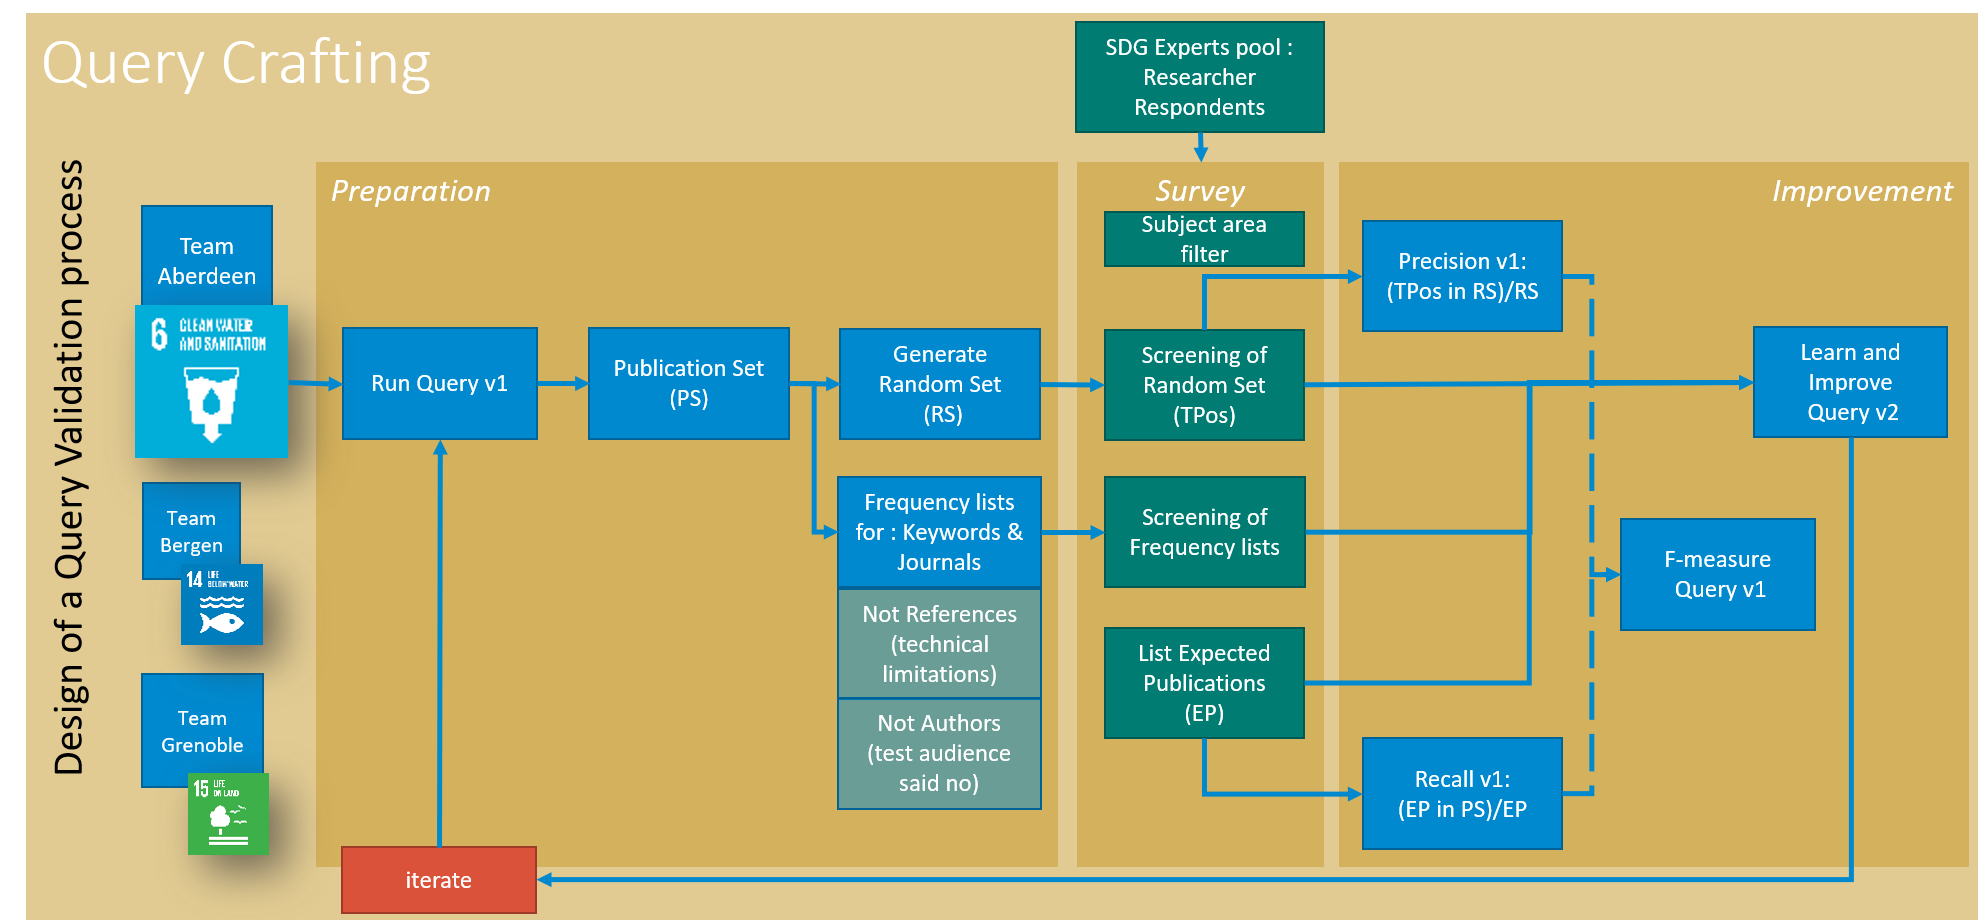
\includegraphics[width=0.9\textwidth]{figures/sdg-query-crafting.png}
	\caption{Workflow for improving Search Queries.}
	\label{improvingsearchqueries}
\end{figure}

It was advised form university leadership that consuming resources for researchers as respondents in a survey is not a path to follow again. This means we are unable to evaluate the precision and recall and make improvements to Version 5 as we have done before. Therefore we need to gain as much as possible from the data already obtained, and using mathematical linguistics models in the future. Therefor we need to make sure we know and evaluate the robustness of the current Version 5 of the Aurora SDG Queries.

\section{Research question}
\label{sec:research-question}

This report will focus on evaluation of the "Aurora SDG Queries" \footnote{\url{https://aurora-network-global.github.io/sdg-queries/} }. We will go into details about the two latest versions of the "Aurora SDG Queries"; comparing version 4 with version 5, and where possible comparing the \emph{Aurora SDG Queries} to the \emph{Elsevier SDG Queries}. And benchmark both using the handpicked "golden" data from the survey. 

\textbf{The main research question we want to answer is:  \\
\emph{What is the quality of the results from the Aurora SDG Queries Version 5?}}

The Precision and Recall is a proven indicator in the Information Retrieval community for assessing the quality of a search result. Precision shows how well do the publications in the results for the SDG search query represent publications that are relevant to that SDG. And Recall shows if the search for that SDG is retrieving all the relevant publications that could possibly exist.

\begin{figure}[ht]
	\centering
  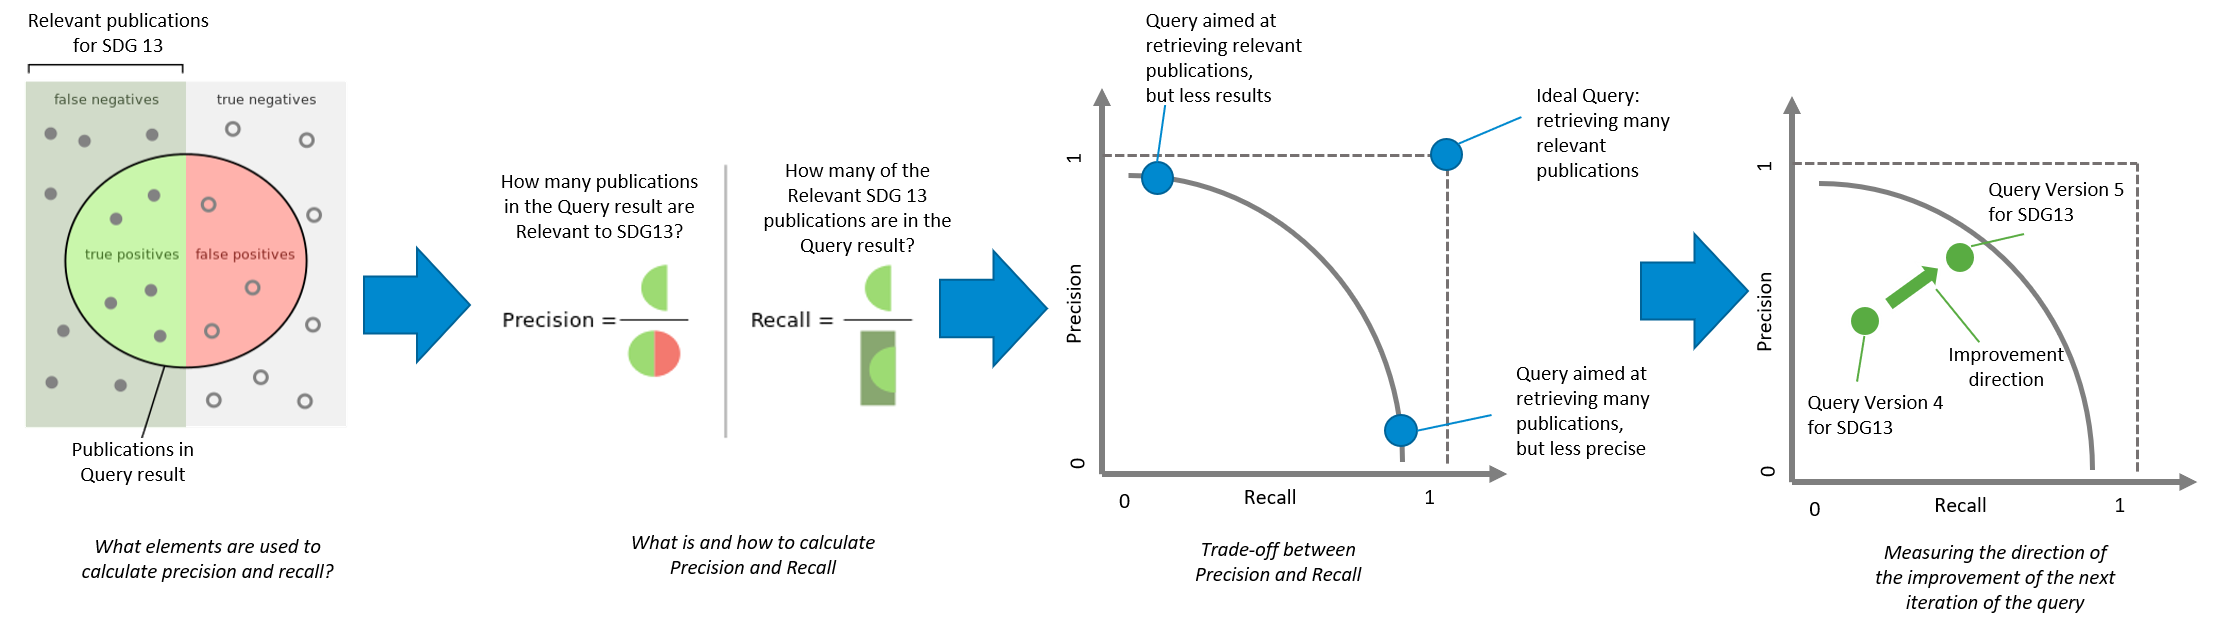
\includegraphics[width=1.0\textwidth]{figures/recall-precision.png}
	\caption{Explanation about Precision and Recall trade-offs and indicators for improvement.}
	\label{precisonandrecallexplanation}
\end{figure}


To answer this question, we need \emph{for Recall} a baseline or "gold" data set with handpicked publications. The more of those publications appear in the research result, the better. This 'gold' data we have from the suggested publication of the survey done earlier in 2020.\cite{vanderfeesten_survey_2020}

Next we need \emph{for Precision} to count the publications from the SDG query result that are relevant. We have done this for the Version 4 Aurora SDG queries using extensive resources from the Aurora Research community. We aren't allowed to do this any more, so we need to work our way around this problem.

We do this by first looking at how much the versions of the SDG queries differ from each other. Not only by size, but by comparing the publications inside each of the SDG collections.

Where the results from the versions do not differ much, we believe the Precision will not change much either. \\
However, where the result do change a lot between the SDG's of the different versions, we need to re-establish the precision again. We do this by getting a random sample from the Version 5 result of an SDG, and let that result evaluate by a bibliometrician familiar with the topic.

\section{Sub-questions, Methods and Results}
In this section we will explain the sub-questions, and why it is important to answer the main question. Along with that we explain the calculation method, and show the results.

We collected the data for Aurora SDG query version 4 at a different time, and different time ranges, that we collected the publications from Scopus for version 5. (time ranges for v4: after 2009 before 2019, for v5: after 2009 and before 2020) This means, when comparing both version, we have to keep in mind that there is a difference of publications in the result sets of roughly one year. We accepted this difference, because it is time consuming to collect all the data from Scopus. 

\subsection{Volume of Publications in SDG result sets}
To get a basic understanding of the data, we take a look at the volume, the number of publications that are we get in each of the versions of the Aurora SDG Queries and the Elsevier SDG Queries.

%=== WHY HOW RESULT ============================================================================

\subsubsection{Amount of Publications per SDG}
We want to know \emph{What are the total number of publications per SDG in the Aurora SDG queries v4 and v5?} and \emph{What are the total number of  publications per SDG, in the Elsevier SDG queries 2020 and 2021?}

To get the total numbers we have ran the  SDG queries for each SDG Target, collected the Scopus Electronic Identifiers (EID's) that occur in each SDG target result sets. We deduplicated the EID's when combined the targets for comparing  each SDG Goal. Then we counted the EID's in each of the SDG query result sets.

The total of the publications collected in the SDG result sets is 1,743,649 publications for the Aurora SDG queries version 4, and 1,555,477 for version 5.

In the figure \ref{numberofresults}, we see the number of publications for each SDG result set ranges from 12,615 in SDG 17 of the Aurora version 4, to 473,190 in SDG 13 of version 5.

More detailed numbers for each SDG result set for each Query version can be found in table \ref{venndataofpublications}.

\begin{figure}[ht]
	\centering
  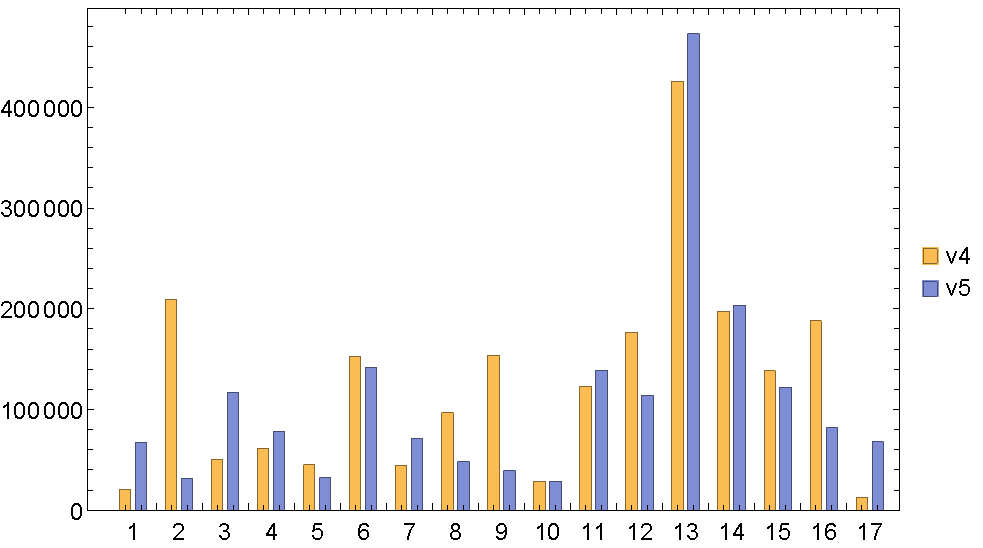
\includegraphics[width=0.75\textwidth]{figures/numberofresultsv4vsv5.pdf}
	\caption{Number of results per SDG for v4 and v5 queries}
	\label{numberofresults}
\end{figure}

We see there is are some SDG result sets that differ a lot, when looking at the volume alone, but also the within a result set might have comparable sises, the publications occurring inside these sets might differ. More about the robustness can be read in section \ref{sec:robustness}.

%=== WHY HOW RESULT ============================================================================

\subsubsection{Amount of SDG labels per Publication}
Next we want to know how well the publications in the SDG result sets are overlapping with other SDG result sets, or are differ from each other.  
We need to know this to see how well the SDG result sets can be used for Machine Learning. The more the classes can be distinguished from each other, the better the model can be trained to distinguish between each of the classes later on in the process.

We want to know \emph{How much and what percentage of the publications have only one SDG label, two SDG labels, etc. in the Aurora SDG queries v4 and v5 ? } and \emph{How much and what percentage of the publications have only one SDG label, two SDG labels, etc. in the Elsevier SDG queries 2020 and 2021?}

Therefore we are looking at how much publications are appearing in one SDG result set, or are appearing in more than one. 

In table \ref{multipleSDG's} we can see that 82.5\%  of the publications in the Aurora SDG Queries version 4 are occurring on only one SDG result set, and 17.5\% of the publications appear in two or more SDG result sets.\\
For the Aurora SDG Queries version 5 we can see that 84.2\% of the publications are occurring on only one SDG result set, and 15.8\% of the publications appear in two or more SDG result sets.\\
This means that the majority of the publications can be used for machine learning, which requires a large corpus for training, 1.3 million papers in case of the version 5 queries.

\begin{table}[H]
 \begin{tabular}{cllll}
 \toprule
 number of SDGs & number of publications (v4) & relative v4 & number of publications (v5) & relative v5 \\
 \hline
 1 & 1438591 & 82.5046 & 1310016 & 84.2196 \\
 2 & 244905 & 14.0455 & 199885 & 12.8504 \\
 3 & 46756 & 2.6815 & 37284 & 2.39695 \\
 4 & 10642 & 0.610329 & 6715 & 0.4317 \\
 5 & 2251 & 0.129097 & 1281 & 0.082 \\
 6 & 408 & 0.023 & 230 & 0.015 \\
 7 & 82 & 0.0047 & 50 & 0.0032 \\
 8 & 12 & 0.00069 & 12 & 0.00077 \\
 9 & 1 & 0.000057 & 2 & 0.00013 \\
 10 & 0 & 0 & 1 & 0.000064 \\
 11 & 1 & 0.000057 & 1 & 0.000064 \\
 \bottomrule
\end{tabular} \caption{Number of publications classified to multiple SDG's for v4 and v5 queries (absolute and relative numbers).}
\label{multipleSDG's}
\end{table}

\begin{figure}[H]
	\centering
  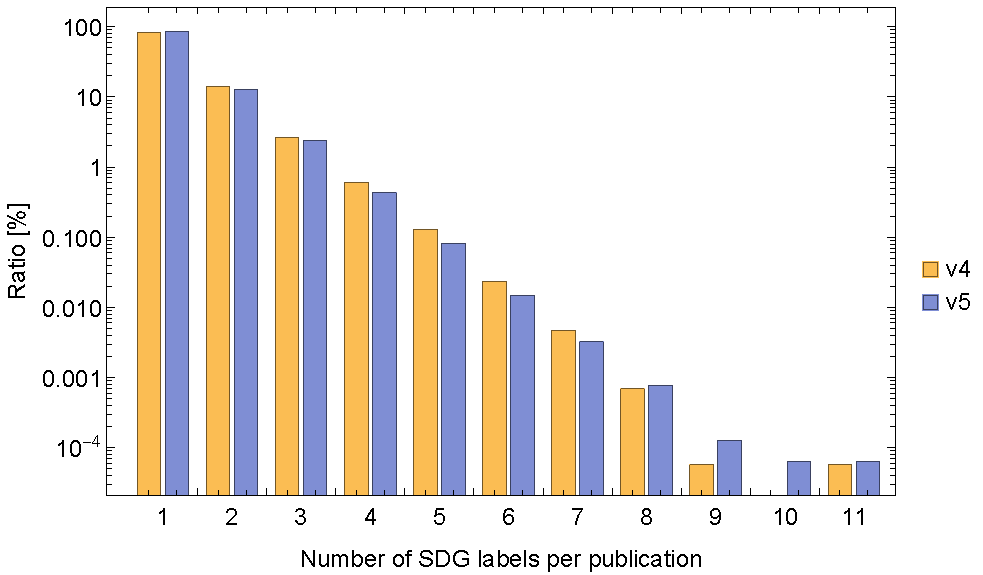
\includegraphics[width=0.75\textwidth]{figures/histogram-multipleSDGlabels-barchartv4+v5.pdf}
	\caption{On logarithmic scale: Percentage of publications classified to one or multiple SDG's for v4 (orange) and v5 (purple) queries.}
\end{figure}

%=== WHY HOW RESULT ============================================================================
\subsection{Overlap of publications between SDG's, within the same SDG query model}

\subsubsection{Overlap within Aurora SDG queries v4 and v5}
In this section we look at the ~20\% of publications that appear in two or more SDG result sets. We now know that more than ~80\% of the publications occur in only one SDG result set. In this section we want to know how that ~20\% looks like. We want to see what the effect is of the publications occurring in multiple SDG's.

We want to know \emph{What is the overlap in numbers of publications of the result sets of the different queries of each SDG, withing version 4 and within version 5 queries? Where do they relatively occur the most? What about the overlap between the targets?}

As you have seen before, the volumes of the publications in the SDG result sets differ in sizes. To compare the overlap between SDG result sets that have different sizes, we need to normalize both the SDG result sets we are comparing. For normalization we used this formula:

\begin{equation*}
    \left.\text{normalized overlap}\right|_{i,j} = \frac{\text{number of publications in SDG i AND j}}{\text{number of publications in SDG i OR j}}\cdot 100\%
\end{equation*}

Here we divide the intersection over the union for the 289 (= 17x17) SDG result set combinations we are comparing. 
We calculate the intersection ("AND") for each  SDG result sets i AND j that we are comparing. This gives us the number of publications that both sets share.
We calculate the union ("OR") for each  SDG result sets i OR j that we are comparing. This gives us the total number of publications in both sets together.

\begin{figure}[H]
	\centering
  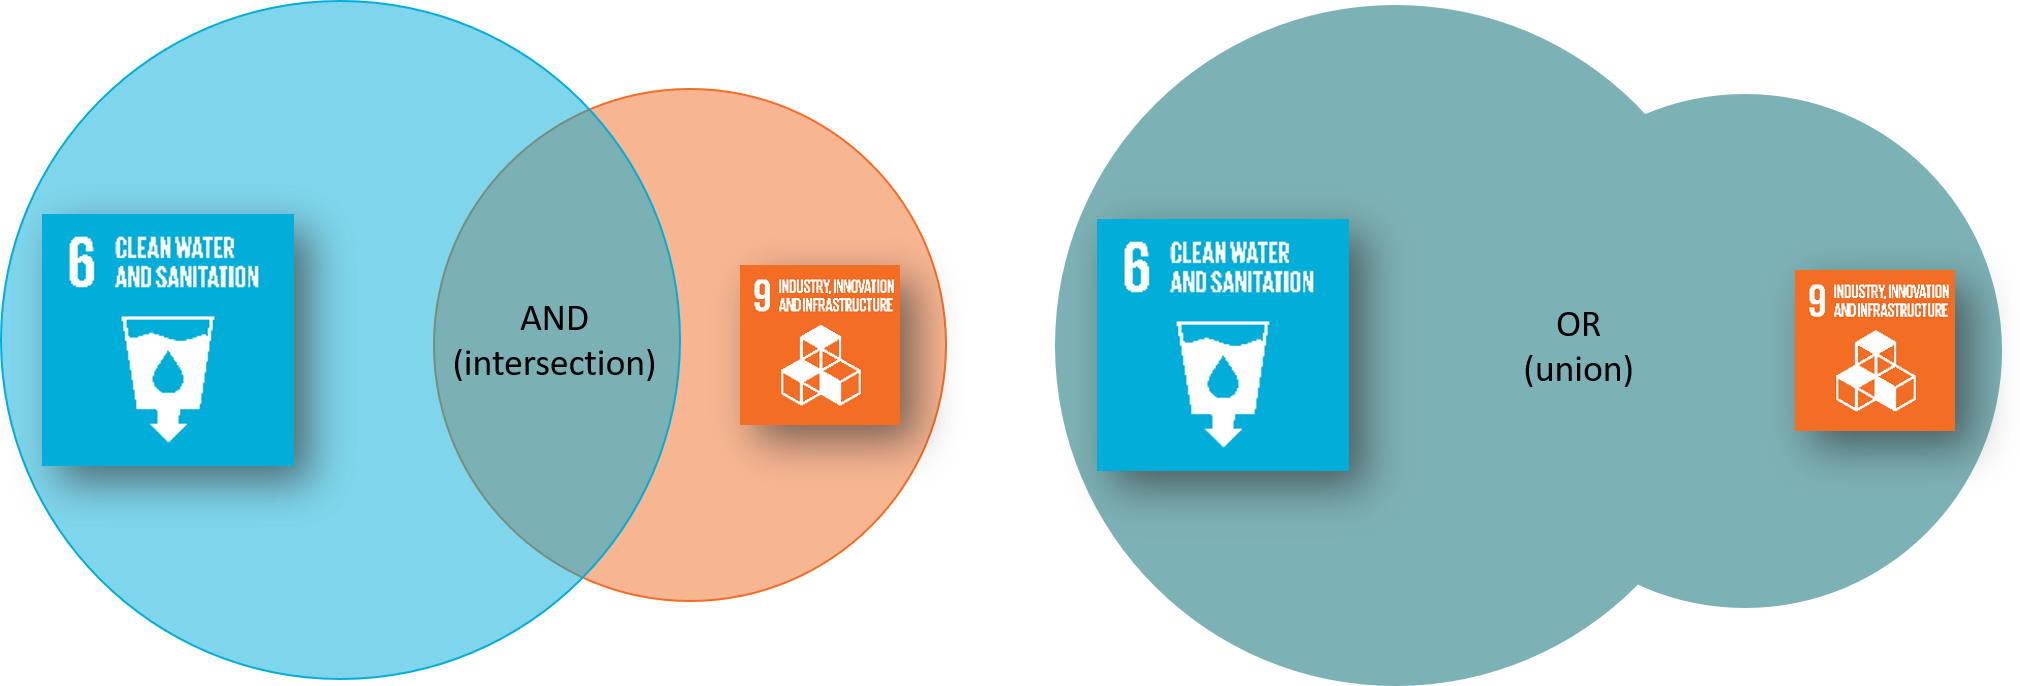
\includegraphics[width=0.75\textwidth]{figures/SDG-OR-AND-venn-diagrams.png}
	\caption{explanation of what is the union and intersection of the SDG result sets.}
\end{figure}

The result is a percentage, where 100\% means that all publications in the SDG i result set will also appear in the SDG j result set. In the histograms below, you see values between 0.014\% and 8.8\%. The higher the number the more overlap between a crossing SDG. \footnote{
Note: We put a 0 on the diagonal line crossing SDG i with SDG i, where there actually should be 100. Because the number of publications that share different SDG's are so small, for proper color-grading the heat-map, }

In figure \ref{heatmapoverlapv4} we see the heat-map for the overlap between different SDG's for the v4 queries. Here you can see that SDG 14 (live below water) and 13 (climate action) share relatively the most publications (8.8\%) and SDG 6 (clean water and sanitation) and 5 (gender equality) the least overlap (0.028\%).

\begin{figure}[H]
    \centering
    \begin{subfigure}{0.49\textwidth}
        \centering
        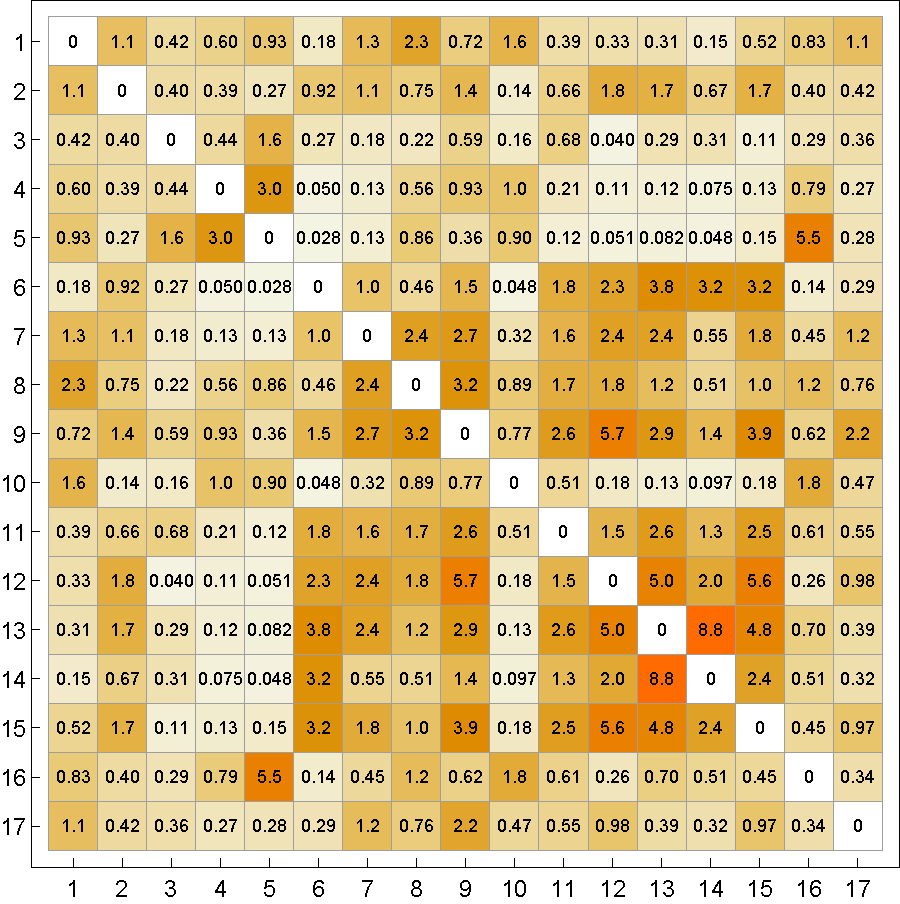
\includegraphics[width=\textwidth]{figures/heatmapv4.pdf}
	    \caption{Overlap of Aurora SDG queries v4. (This represents 17.5\% of publications labeled with more than one SDG.)}
	    \label{heatmapoverlapv4}
    \end{subfigure}
    \hfill
    \begin{subfigure}{0.49\textwidth}
        \centering
        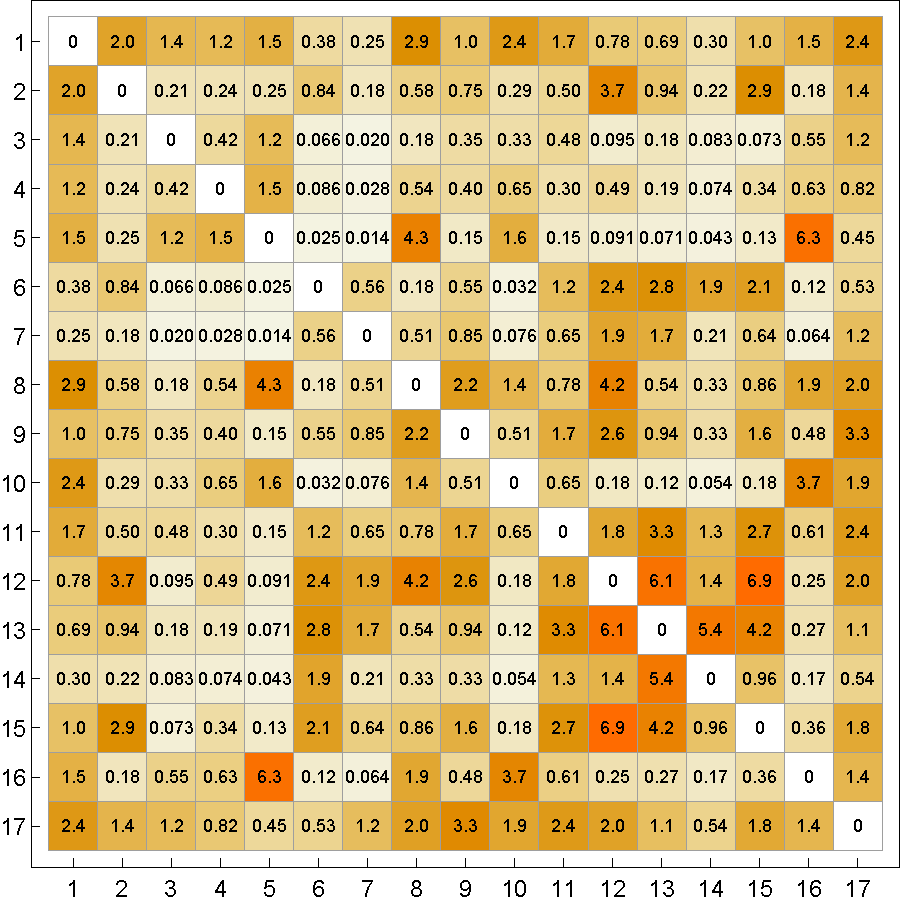
\includegraphics[width=\textwidth]{figures/heatmapv5.pdf}
	    \caption{Overlap of Aurora SDG queries v5. (This represents 15.8\% of publications labeled with more than one SDG.)}
	    \label{heatmapoverlapv5}
    \end{subfigure}
    \caption{Heat-map for the overlap (in \%) between different SDG's.}
\end{figure}


% \begin{figure}[H]
% 	\centering
%   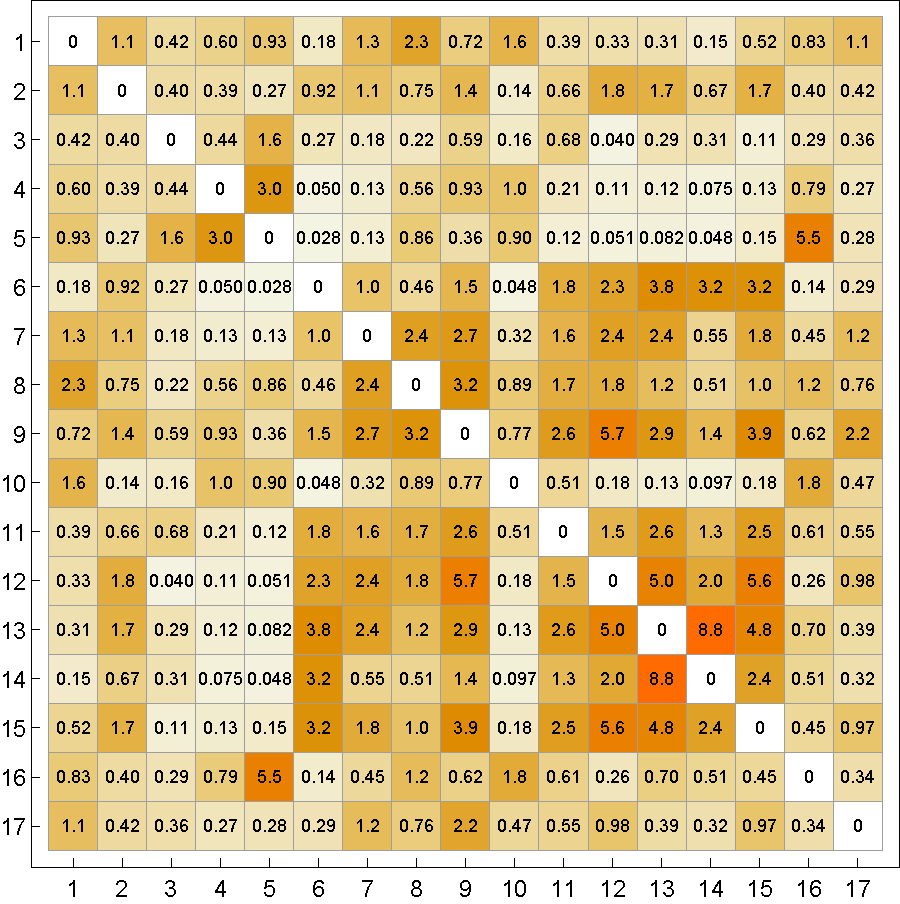
\includegraphics[width=0.75\textwidth]{figures/heatmapv4.pdf}
% 	\caption{Heat-map for the overlap (in \%) between different SDG's for v4 queries. (This diagram represents only the 17.5\% of the publications that are labeled with more than one SDG.)}
% 	\label{heatmapoverlapv4}
% \end{figure}

In  figure \ref{heatmapoverlapv5} we see the heat-map for the overlap between different SDG's for the v5 queries. Here you can see that SDG 12 (responsible consumption and production) and 15 (life on land) share relatively the most publications (6.9\%) and SDG 7 (clean energy) and 5 (gender equality) the least overlap (0.014\%)

% \begin{figure}[H]
% 	\centering
%   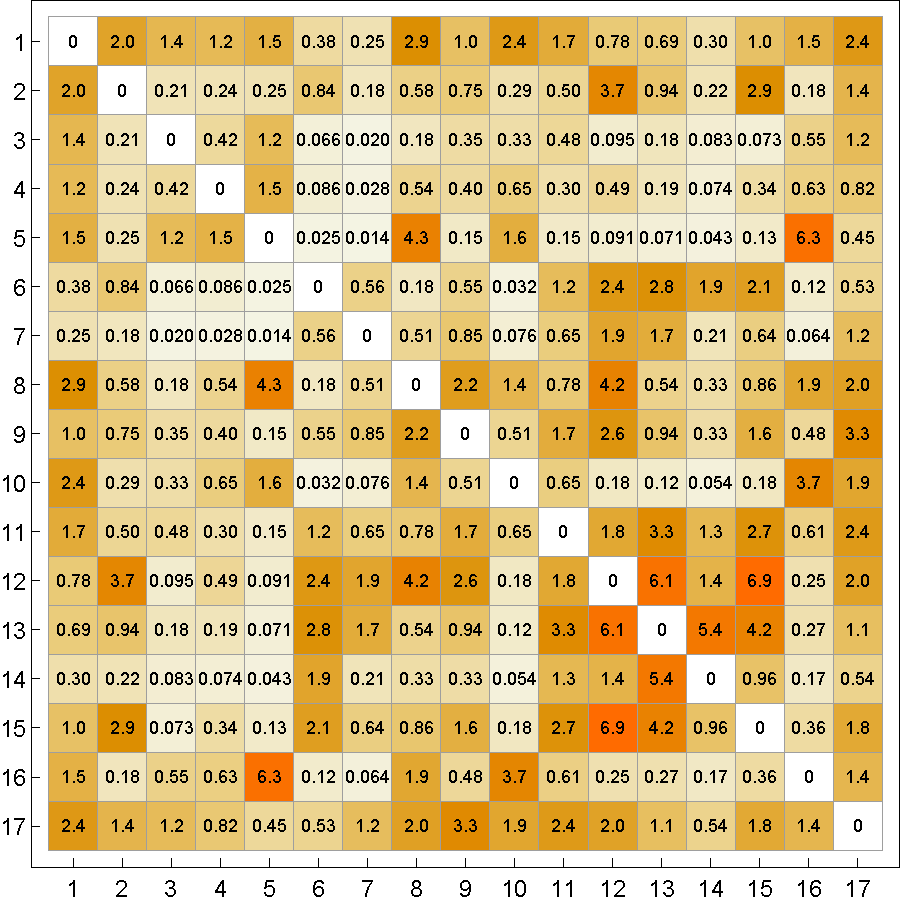
\includegraphics[width=0.75\textwidth]{figures/heatmapv5.pdf}
% 	\caption{Heatmap for the overlap (in \%) between different SDG's for v5 queries. (This diagram represents only the 15.8\% of the publications that are labeled with more than one SDG.)}
% 	\label{heatmapoverlapv5}
% \end{figure}

%\begin{figure}[H]
%	\centering
%  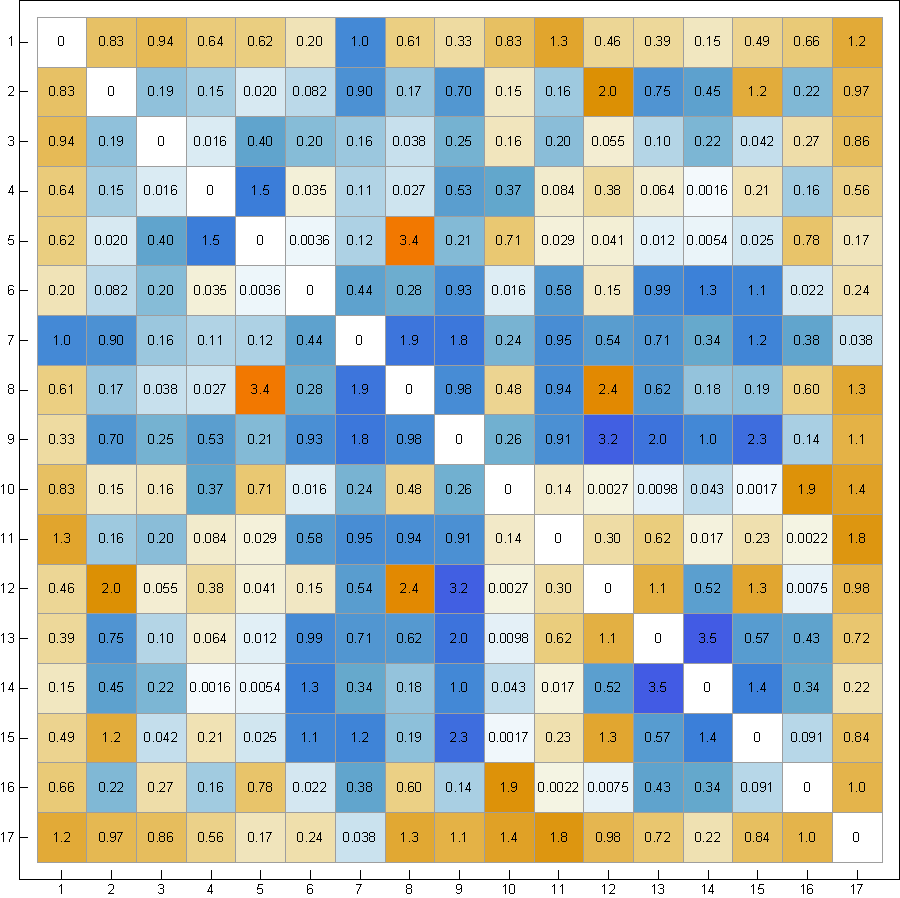
\includegraphics[width=0.75\textwidth]{figures/heatmapdiff.pdf}
%	\caption{Change of the relative overlap from v4 to v5.}
%	\label{heatmapoverlapdiff}
%\end{figure}

With a maximum overlap of 8.8\% within the 15.8\% of multi-labeled publications, we can conclude that the overlap between publication in the SDG result sets are very small. Invertedly this means that the differences between the SDG's are big enough. This is helpful information that gives us confidence that we can define clear classes in the corpus of publications which is very useful for machine learning. This enables us to train a text-classifier that is able to distinguish a text on the level of these 17 SDG Goals.

\paragraph{Overlap on the level of the targets withing Aurora SDG queries v5}
Next we want to look deeper in the 15.8\% of the publications with overlap of the Aurora SDG queries v5, and see the how much of the targets show overlap. We have created 170 sub-queries, one for each of the targets in the 17 Goals. We want to know how much of the publications in the result set for target 1.1 appears also in target 1.2, etc. We also look at the targets outside the parent SDG goal, where we want to know how much of the publications in the result set for target 1.1 appears in target 13.4, etc. This makes up to 14,365 combinations for the overlap between the targets.

We want to know how big the overlap is of the publications on the level of the targets. We have calculated this by looking at the percentage of publication that show overlap between SDG target i.x and SDG target j.y. Than we have created buckets of 0.1\%, so we see the percentage of the 14,365target combination that share publications  0\% till 0.1\% overlap, from 0.1\% till 0.2\%, etc. We limited the buckets to 5\%.

In figure \ref{subquerieshistogram} we see a histogram of the target sub-queries. Here we see that 84\% of the 14365 possible combinations of the sub-queries have an overlap of less than 0.1\%. Than the overlap drops drastically; the second bar is already at 9\% of the publications show an overlap between 0.1 and 0.2\%.

\begin{figure}[H]
	\centering
  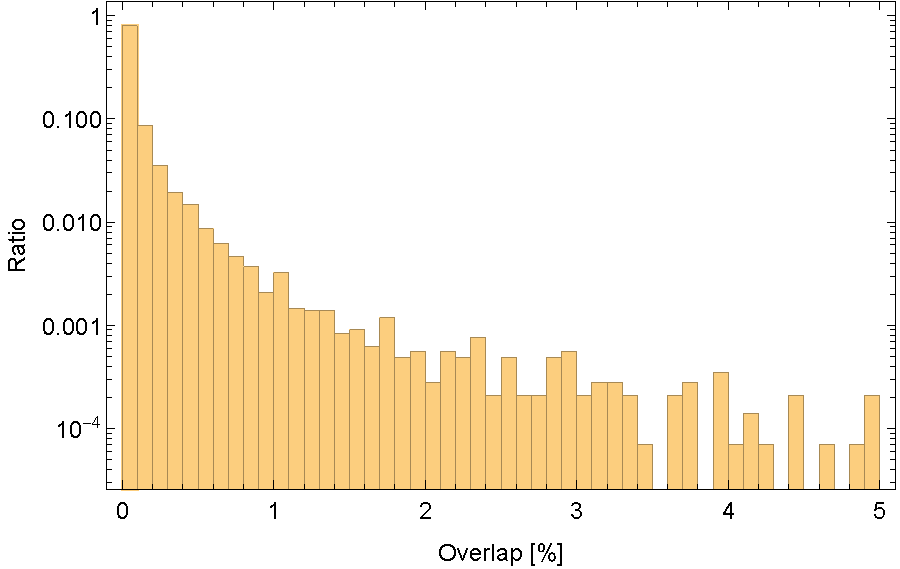
\includegraphics[width=0.75\textwidth]{figures/subqueryhistogram.pdf}
	\caption{Histogram of the target subqueries. 80\% of the 14365 possible combinations of the subqueries have an overlap of less than 0.1\%.}
	\label{subquerieshistogram}
\end{figure}

Next, we want to know in more detail, what the targets are that overlap the most and why.

In  figure \ref{heatmapoverlapv5subqueries} we see the heat-map with 14,365 combinations for the overlap between the 170 Targets within the 17 SDG's for the v5 queries. 

\begin{figure}[H]
	\centering
  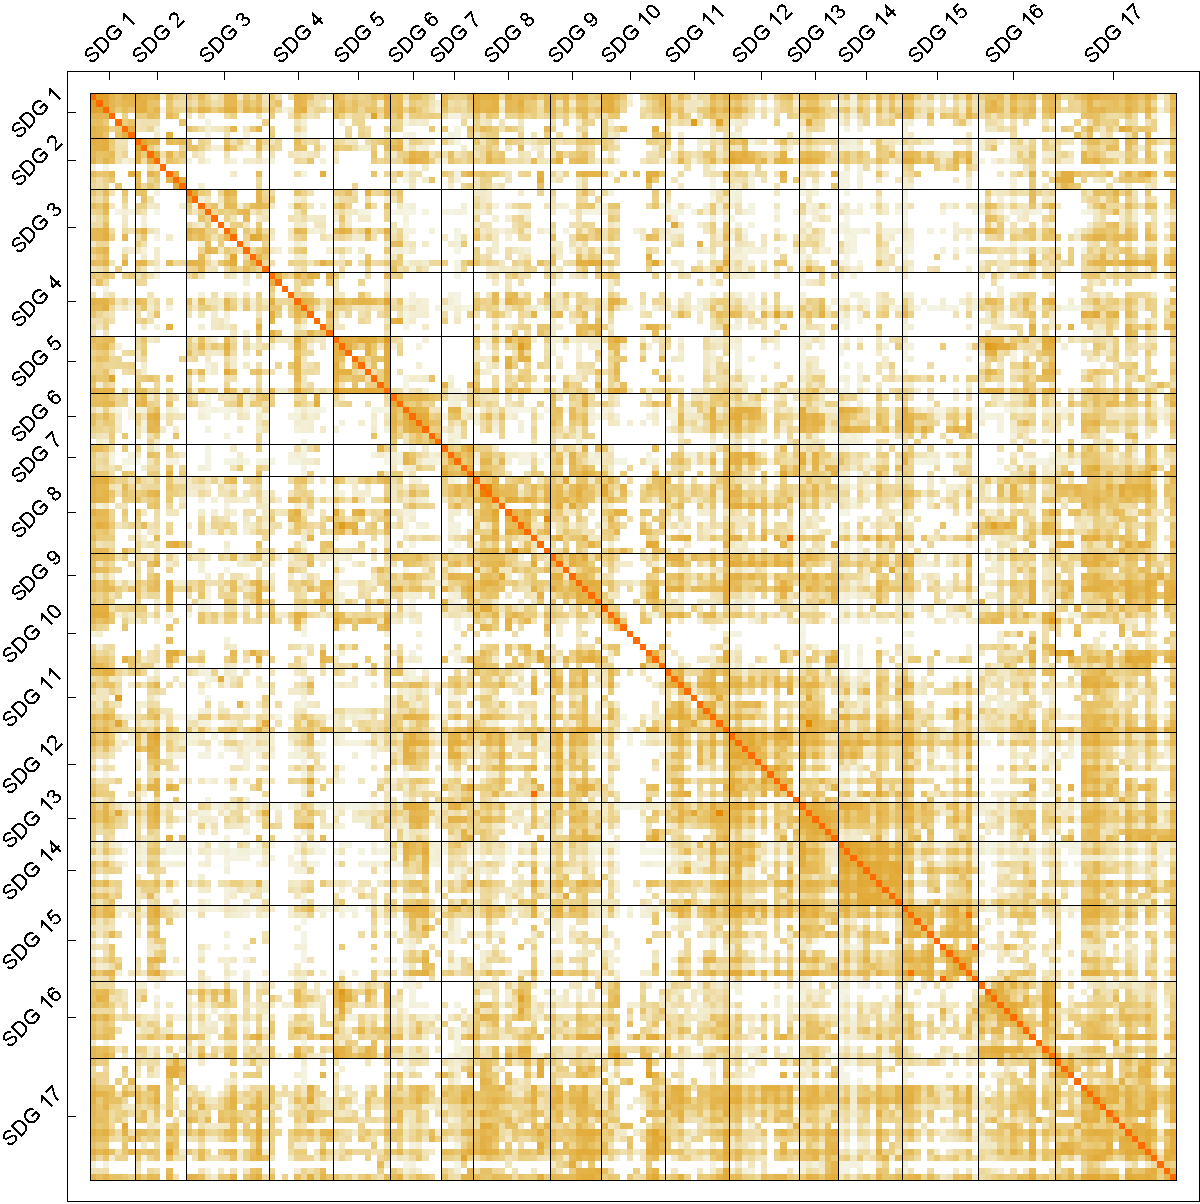
\includegraphics[width=0.75\textwidth]{figures/overlap_per_subquery.pdf}
	\caption{Heatmap for the overlap between different Targets of the SDG's for v5 queries.}
	\label{heatmapoverlapv5subqueries}
\end{figure}

Here in figure \ref{heatmapoverlapv5subqueries} you can see the dark orange dots on the diagonal lines, this shows that the most overlap of publications occurs within the same target. In the rest of the diagram we see a field of orange colors. We see that the targets within the SDG 14 show relatively the most overlap. Also some bright dark orange dots in the more remote areas of the diagonal line. Zooming in to one of those we see that between targets outside an SDG that target 8.9 and 12.b share almost the identical same publications.

When we investigate the sub- queries for those targets, we can see that they share a query line that is identical, which probably takes account for the majority of the publications in that result set.

Sub-query for Target 8.9 in\footnote{ Source: \url{https://aurora-network-global.github.io/sdg-queries/query_SDG8.xml}} Aurora SDG queries v5: 
\begin{quote}
\begin{verbatim}
TITLE-ABS-KEY(("sustaina*") W/3 ("tourism")) OR 
TITLE-ABS-KEY(("GDP" OR "Gross Domestic Product") W/3 ("tourism")) OR 
TITLE-ABS-KEY(("job*") W/3 ("tourism"))
\end{verbatim}
\end{quote}

Sub-query for Target 12.b in\footnote{ Source: \url{https://aurora-network-global.github.io/sdg-queries/query_SDG12.xml}} Aurora SDG queries v5:
\begin{quote}
\begin{verbatim}
TITLE-ABS-KEY((("sustainab*") W/3 ("tourism*")))
\end{verbatim}
\end{quote}

We can conclude that the overlap between publication in the Target sub-query  result sets are very small. This means that the differences between the SDG's are big enough, so we have clear classes in the corpus of publications that is very useful for machine learning. This enables us to train a text-classifier that is able to distinguish a text on the level of these 17 SDG Goals.

%=== WHY HOW RESULT ============================================================================

\subsubsection{Elsevier SDG queries v2020 vs. v2021}
The following section focuses a bit on the Elsevier Queries, where we have a partnership with their teams. in 2019 Elsevier, lead by Bamini, created the initial version of the SDG queries version 2020 as an assignment by Times Higher Education as  part for their new Impact Ranking. \cite{jayabalasingham_identifying_2019}
The 2021 version is a different version, created by Science Metrix, lead by Maxime Rivest. \cite{rivest_improving_2021} This version is different because their starting point were mini-queries their used in another use case for UNESCO. they improved the queries a bit using the Aurora SDG queries, and extended the recall a bit by using a citation graph model.


We want to know what is the overlap in numbers of publications of the result sets of the different queries of each SDG, between Elsevier SDG queries \footnote{Elsevier SDG Queries only account for 16 of the SDG's. } version 2020 and version 2021?

Maxime calculated the difference between the result sets and plotted them in venn diagrams.

\begin{figure}[H]
    \centering
    \begin{subfigure}{0.24\textwidth}
        \centering
        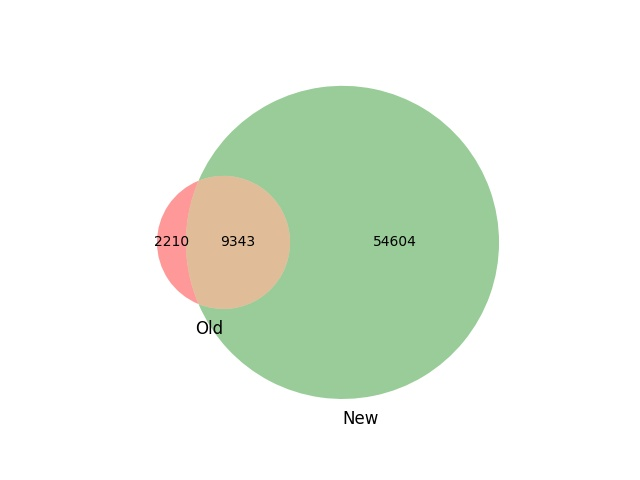
\includegraphics[width=\textwidth]{figures/aurora-elsevier-venn/venn_sdg_1.jpg}
	    \caption{SDG 1}
    \end{subfigure}
    \hfill
    \begin{subfigure}{0.24\textwidth}
        \centering
        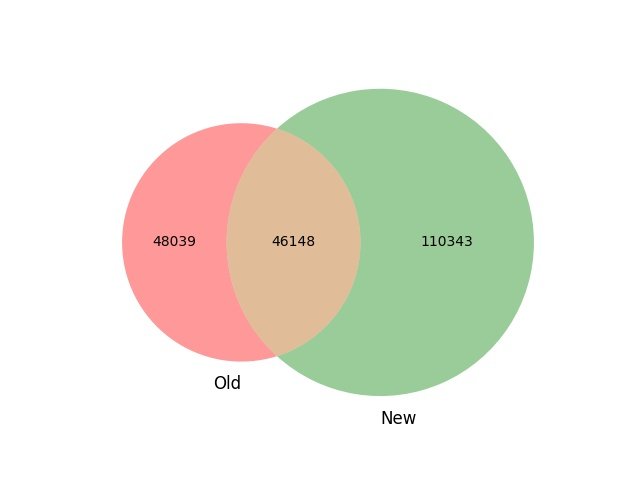
\includegraphics[width=\textwidth]{figures/aurora-elsevier-venn/venn_sdg_2.jpg}
	    \caption{SDG 2}
    \end{subfigure}
    \hfill
    \begin{subfigure}{0.24\textwidth}
        \centering
        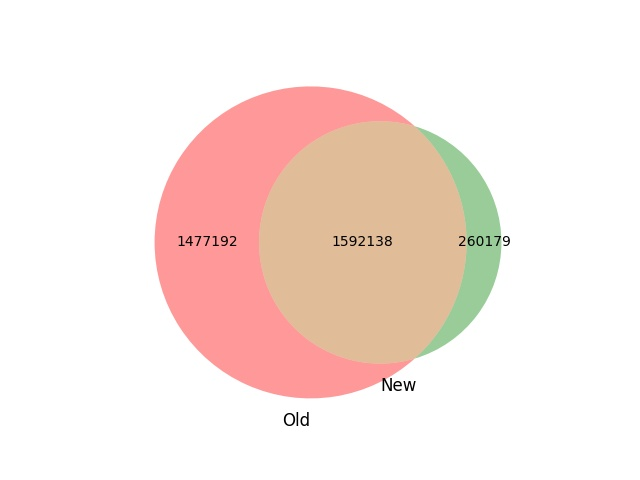
\includegraphics[width=\textwidth]{figures/aurora-elsevier-venn/venn_sdg_3.jpg}
	    \caption{SDG 3}
    \end{subfigure}
    \hfill
    \begin{subfigure}{0.24\textwidth}
        \centering
        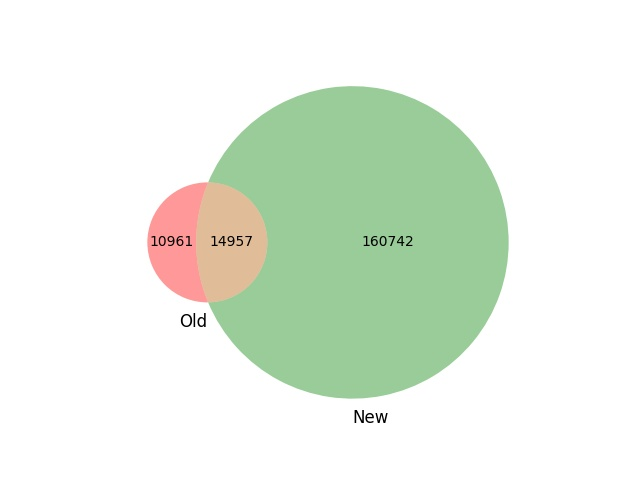
\includegraphics[width=\textwidth]{figures/aurora-elsevier-venn/venn_sdg_4.jpg}
	    \caption{SDG 4}
    \end{subfigure}
    % ROW
    \begin{subfigure}{0.24\textwidth}
        \centering
        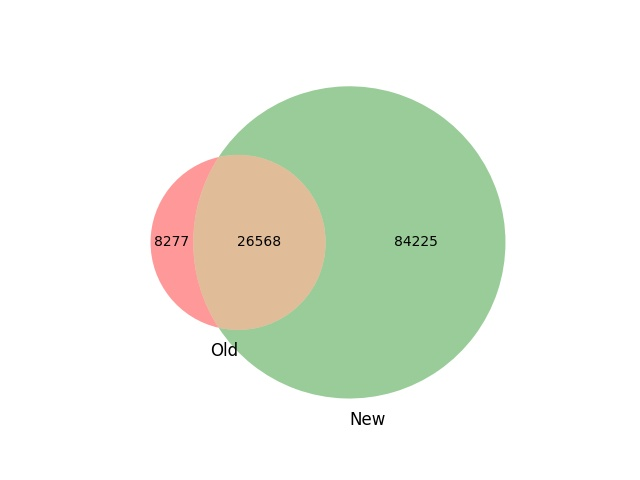
\includegraphics[width=\textwidth]{figures/aurora-elsevier-venn/venn_sdg_5.jpg}
	    \caption{SDG 5}
    \end{subfigure}
    \hfill
    \begin{subfigure}{0.24\textwidth}
        \centering
        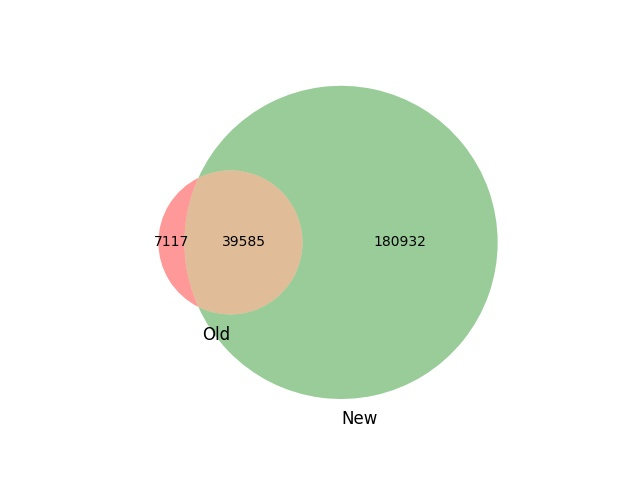
\includegraphics[width=\textwidth]{figures/aurora-elsevier-venn/venn_sdg_6.jpg}
	    \caption{SDG 6}
    \end{subfigure}
    \hfill
    \begin{subfigure}{0.24\textwidth}
        \centering
        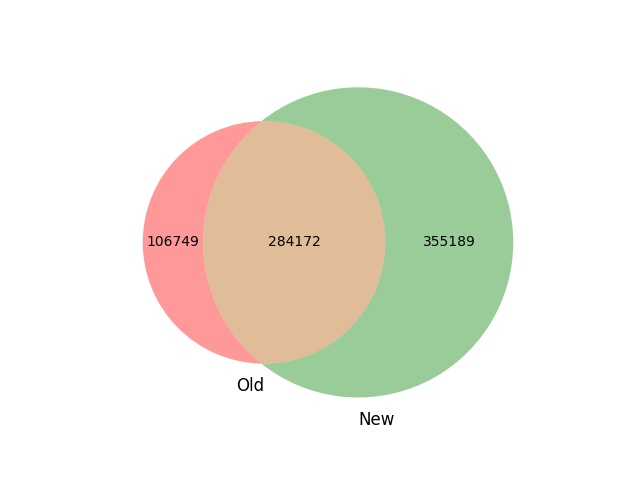
\includegraphics[width=\textwidth]{figures/aurora-elsevier-venn/venn_sdg_7.jpg}
	    \caption{SDG 7}
    \end{subfigure}
    \hfill
    \begin{subfigure}{0.24\textwidth}
        \centering
        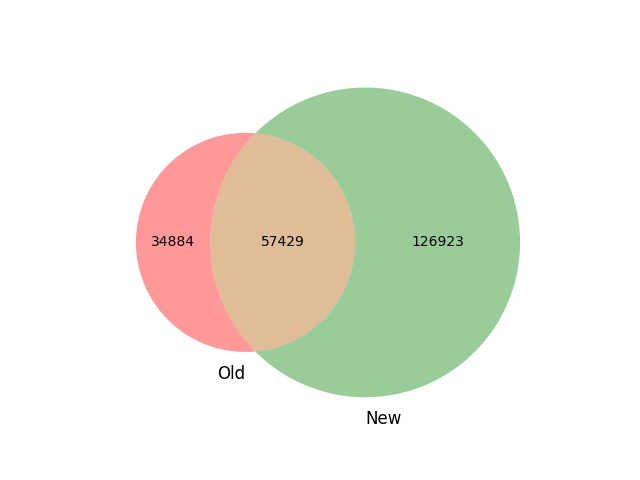
\includegraphics[width=\textwidth]{figures/aurora-elsevier-venn/venn_sdg_8.jpg}
	    \caption{SDG 8}
    \end{subfigure}
    % ROW
        \begin{subfigure}{0.24\textwidth}
        \centering
        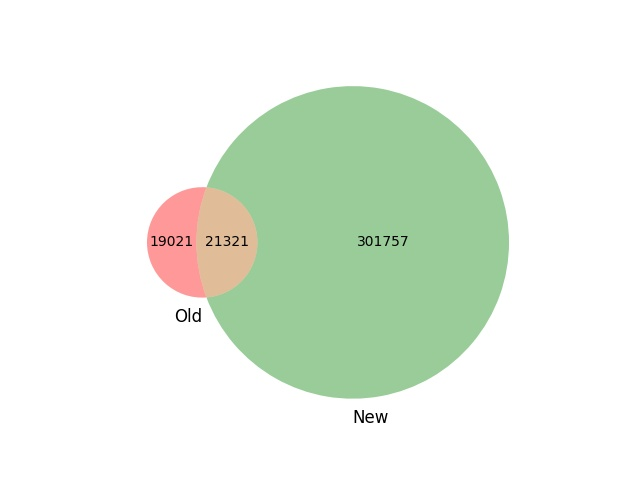
\includegraphics[width=\textwidth]{figures/aurora-elsevier-venn/venn_sdg_9.jpg}
	    \caption{SDG 9}
    \end{subfigure}
    \hfill
    \begin{subfigure}{0.24\textwidth}
        \centering
        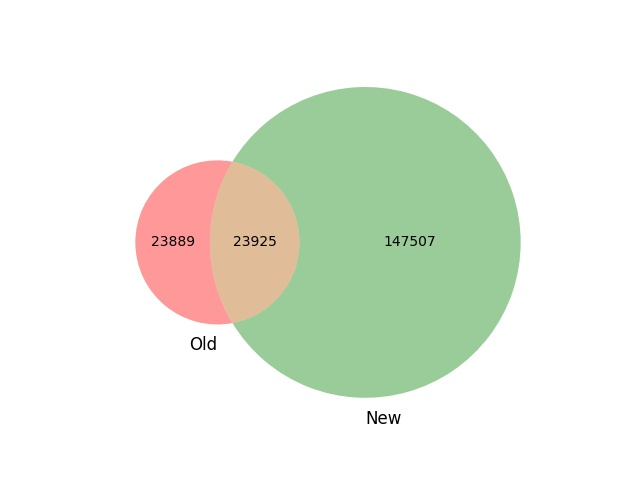
\includegraphics[width=\textwidth]{figures/aurora-elsevier-venn/venn_sdg_10.jpg}
	    \caption{SDG 10}
    \end{subfigure}
    \hfill
    \begin{subfigure}{0.24\textwidth}
        \centering
        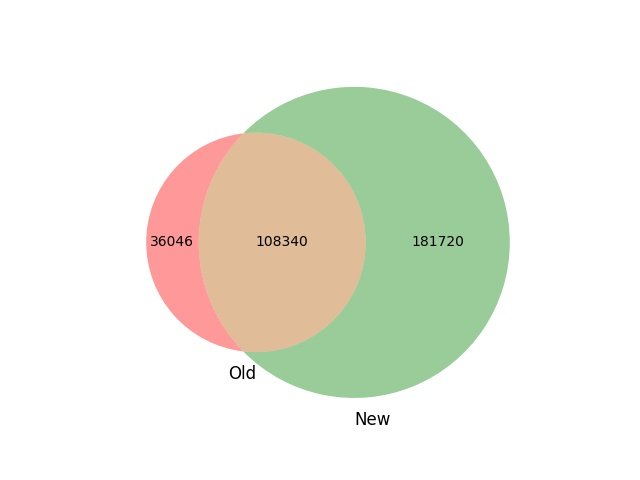
\includegraphics[width=\textwidth]{figures/aurora-elsevier-venn/venn_sdg_11.jpg}
	    \caption{SDG 11}
    \end{subfigure}
    \hfill
    \begin{subfigure}{0.24\textwidth}
        \centering
        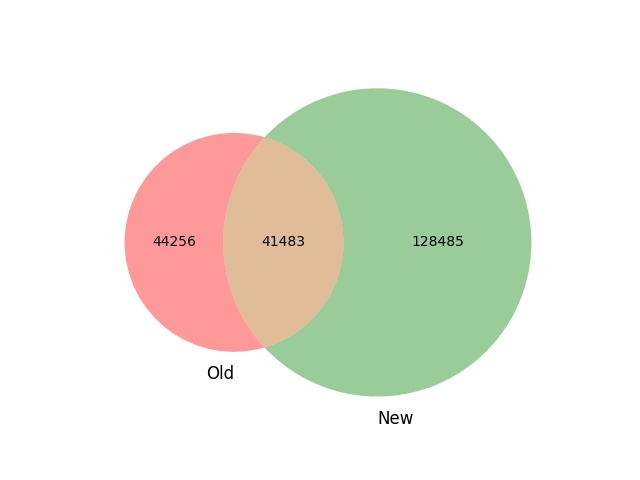
\includegraphics[width=\textwidth]{figures/aurora-elsevier-venn/venn_sdg_12.jpg}
	    \caption{SDG 12}
    \end{subfigure}
    % ROW
        \begin{subfigure}{0.24\textwidth}
        \centering
        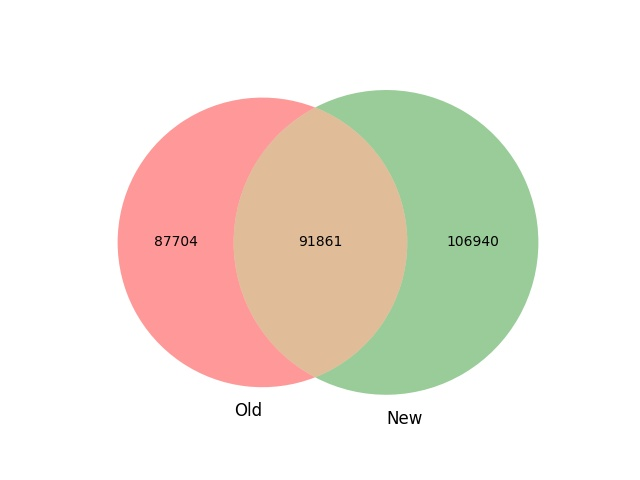
\includegraphics[width=\textwidth]{figures/aurora-elsevier-venn/venn_sdg_13.jpg}
	    \caption{SDG 13}
    \end{subfigure}
    \hfill
    \begin{subfigure}{0.24\textwidth}
        \centering
        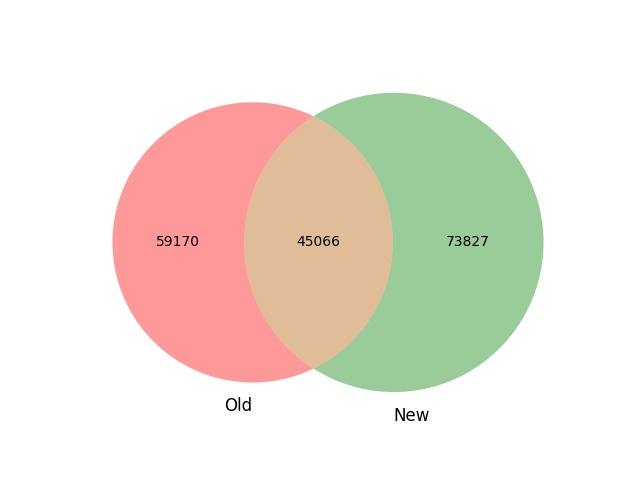
\includegraphics[width=\textwidth]{figures/aurora-elsevier-venn/venn_sdg_14.jpg}
	    \caption{SDG 14}
    \end{subfigure}
    \hfill
    \begin{subfigure}{0.24\textwidth}
        \centering
        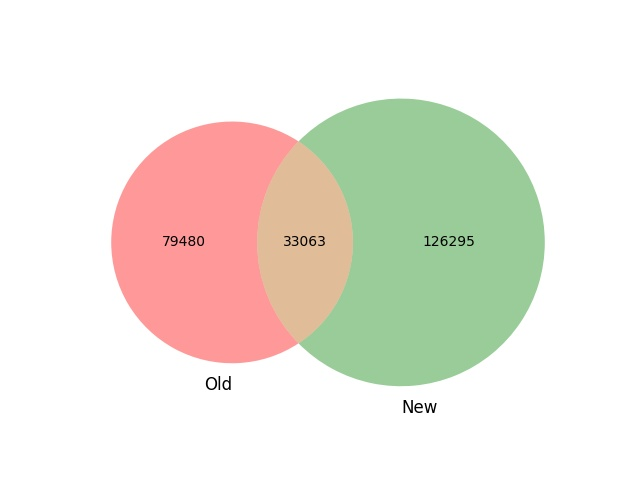
\includegraphics[width=\textwidth]{figures/aurora-elsevier-venn/venn_sdg_15.jpg}
	    \caption{SDG 15}
    \end{subfigure}
    \hfill
    \begin{subfigure}{0.24\textwidth}
        \centering
        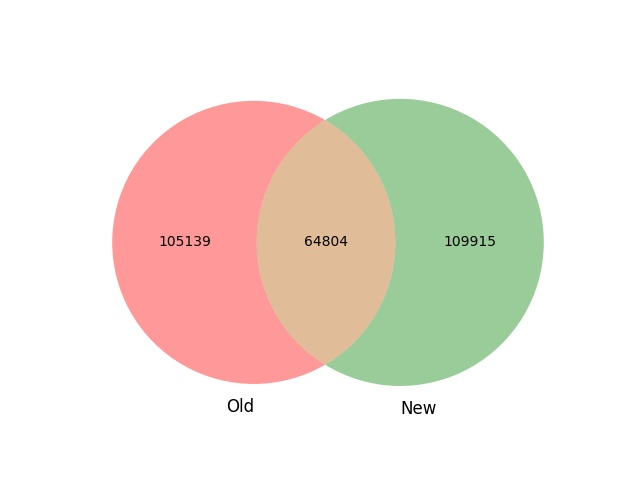
\includegraphics[width=\textwidth]{figures/aurora-elsevier-venn/venn_sdg_16.jpg}
	    \caption{SDG 16}
    \end{subfigure}
    \caption{Differences between Elsevier SDG queries version 2020 (red) and version 2021 (green)}
\end{figure}


%=== WHY HOW RESULT ============================================================================

\subsection{Differences between query models: Aurora SDG queries v5 vs. Elsevier SDG queries v2021}

Next we want to know what the difference is between the latest SDG query models; the Elsevier SDG queries version 2021, and the Aurora SDG queries version 5.

Also here Science Metrix was so kind to share their results.
Used by courtesy of Maxime Rivest (Science Metrix / Elsevier)

\begin{figure}[H]
	\centering
  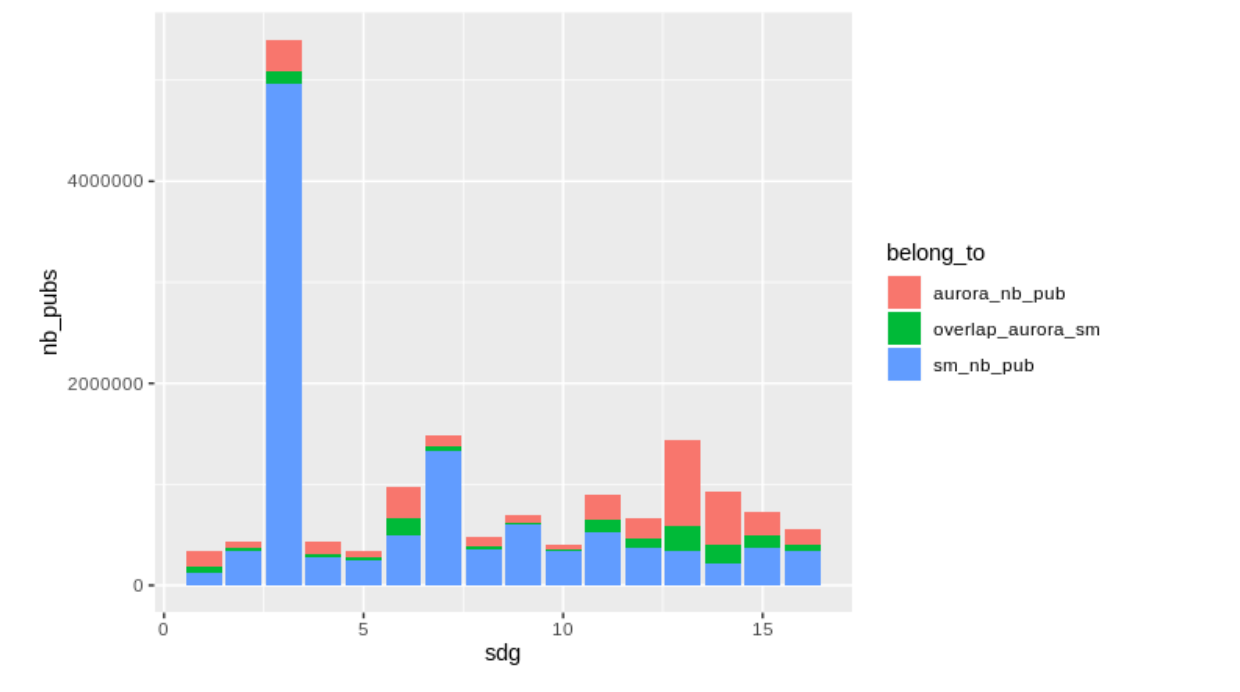
\includegraphics[width=0.75\textwidth]{figures/aurora-elsevier-venn/overlap-aurora-elsevier-absolutes.png}
	\caption{Bar diagrams for the overlap between different SDG query models.  Aurora SDG queries v5 (in Red), Elsevier SDG queries 2021 (in Blue), Overlap (in Green)}
\end{figure}

\begin{figure}[H]
	\centering
  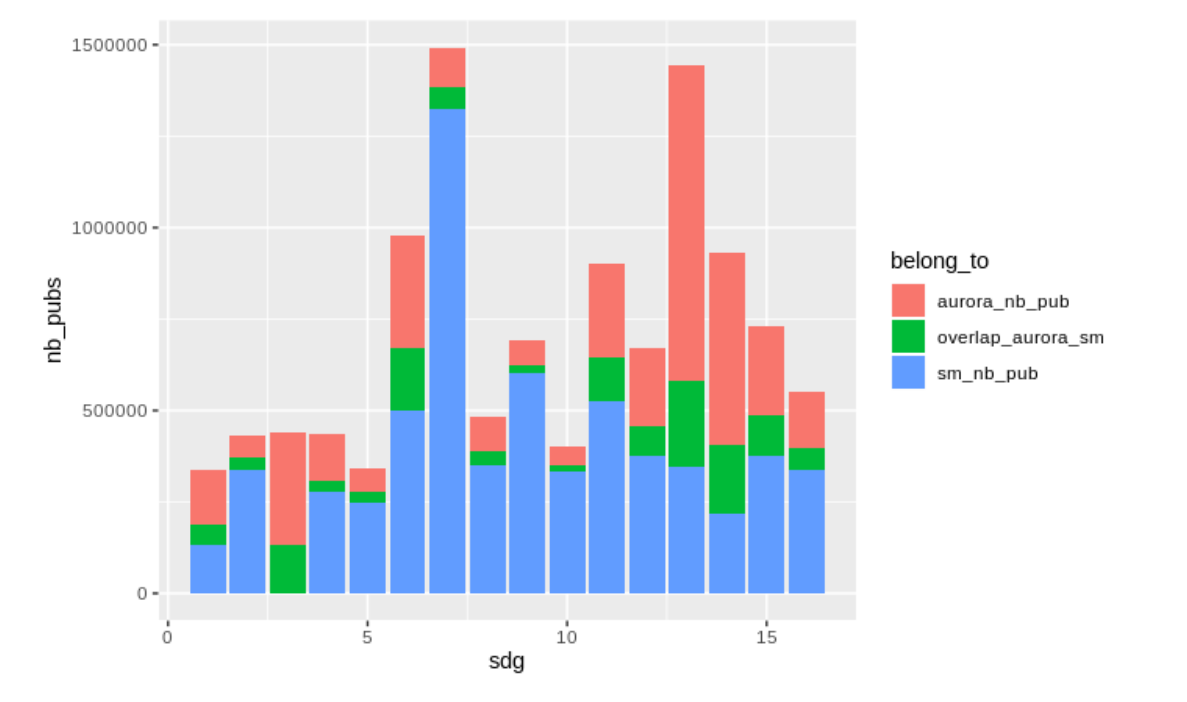
\includegraphics[width=0.75\textwidth]{figures/aurora-elsevier-venn/overlap-aurora-elsevier-absolutes2.png}
	\caption{Bar diagrams for the overlap between different SDG query models, excluding Elsevier's SDG3. Aurora SDG queries v5 (in Red), Elsevier SDG queries 2021 (in Blue), Overlap (in Green)}
\end{figure}

We see in these diagrams that there is overlap between the models, but that overlap is very small, and that the result sets from Elsevier is bigger than those from Aurora. This is due to the fact that both models are created with a different use case in mind.

The Aurora SDG queries aim at precision of the search results, first of all in order to minimise false positives for the use cases to identify researchers in the various Aurora universities institutes related to an SDG and each of the targets. And secondly to create a corpus that can be used for machine learning, to expand the SDG labeling mechanism for research in the local languages of the Aurora universities without re-creating all the queries for the various languages.

The Elsevier SDG queries serve the use case for ranking universities to the Times Higher Education Impact Ranking. Here we can imagine more recall is favored over precision, in order to create a substantial corpus to have the majority of the universities worldwide represented in the ranking.

As being said by Rafols et al. 2021 \cite{rafols_visualising_2021} different stakeholders have different perspectives and needs regarding mapping research papers to the SDG's, and those should be given tools by interactively allowing to make a custom mapping \footnote{\url{https://public.tableau.com/profile/ed.noyons\#!/vizhome/UKStringsSDGtocommunities/Dashboard1}}.

%=== WHY HOW RESULT ============================================================================
% MAURICE WAS HERE
\subsection{Robustness: Change ratio within versions v4 and v5}
\label{sec:robustness}
To get a basic understanding about how the queries changed from v4 to v5 we take a look at the overlap between the results per SDG. Therefore, we calculate the number of publications that are assigned to a SDG for v4 and v5 queries (cardinalities), the number of publications that are assigned to a SDG by both versions of the queries (complements), the number of publications that are assigned only by one version of the queries (intersection) and the number of publications that are assigned to an SDG eiter by v4 or by v5 (union). The results are depicted in Table \ref{venndataofpublications}.
\begin{table}[H]
\centering 
 \begin{tabular}{ccccccc}
 \toprule
  SDG & v4 & v5 & v4 AND v5 & v4 OR v5 & v4 AND NOT v5 & v5 AND NOT v4 \\
  \hline
 1 & 20706 & 67112 & 69234 & 18584 & 2122 & 48528 \\
 2 & 209366 & 31142 & 223205 & 17303 & 192063 & 13839 \\
 3 & 50533 & 116711 & 129729 & 37515 & 13018 & 79196 \\
 4 & 61644 & 78595 & 83424 & 56815 & 4829 & 21780 \\
 5 & 45013 & 32205 & 58773 & 18445 & 26568 & 13760 \\
 6 & 152917 & 141939 & 234176 & 60680 & 92237 & 81259 \\
 7 & 44370 & 71294 & 112219 & 3445 & 40925 & 67849 \\
 8 & 96695 & 48266 & 122169 & 22792 & 73903 & 25474 \\
 9 & 153758 & 39013 & 178146 & 14625 & 139133 & 24388 \\
 10 & 28540 & 28573 & 46027 & 11086 & 17454 & 17487 \\
 11 & 123278 & 138698 & 172822 & 89154 & 34124 & 49544 \\
 12 & 176610 & 113947 & 240985 & 49572 & 127038 & 64375 \\
 13 & 425933 & 473190 & 508246 & 390877 & 35056 & 82313 \\
 14 & 197303 & 203463 & 254179 & 146587 & 50716 & 56876 \\
 15 & 138378 & 122252 & 172419 & 88211 & 50167 & 34041 \\
 16 & 187971 & 82465 & 240962 & 29474 & 158497 & 52991 \\
 17 & 12615 & 67903 & 74710 & 5808 & 6807 & 62095 \\
 all & 1743649 & 1555477 & 2323166 & 975960 & 767689 & 579517 \\
 \bottomrule
\end{tabular}\caption{Number of publications per SDG: v4, v5, intersection between v4 and v5, union of v4 and v5, only in v4, and only in v5.}
\label{venndataofpublications}
\end{table}
%\begin{figure}[H]
%	\centering
%  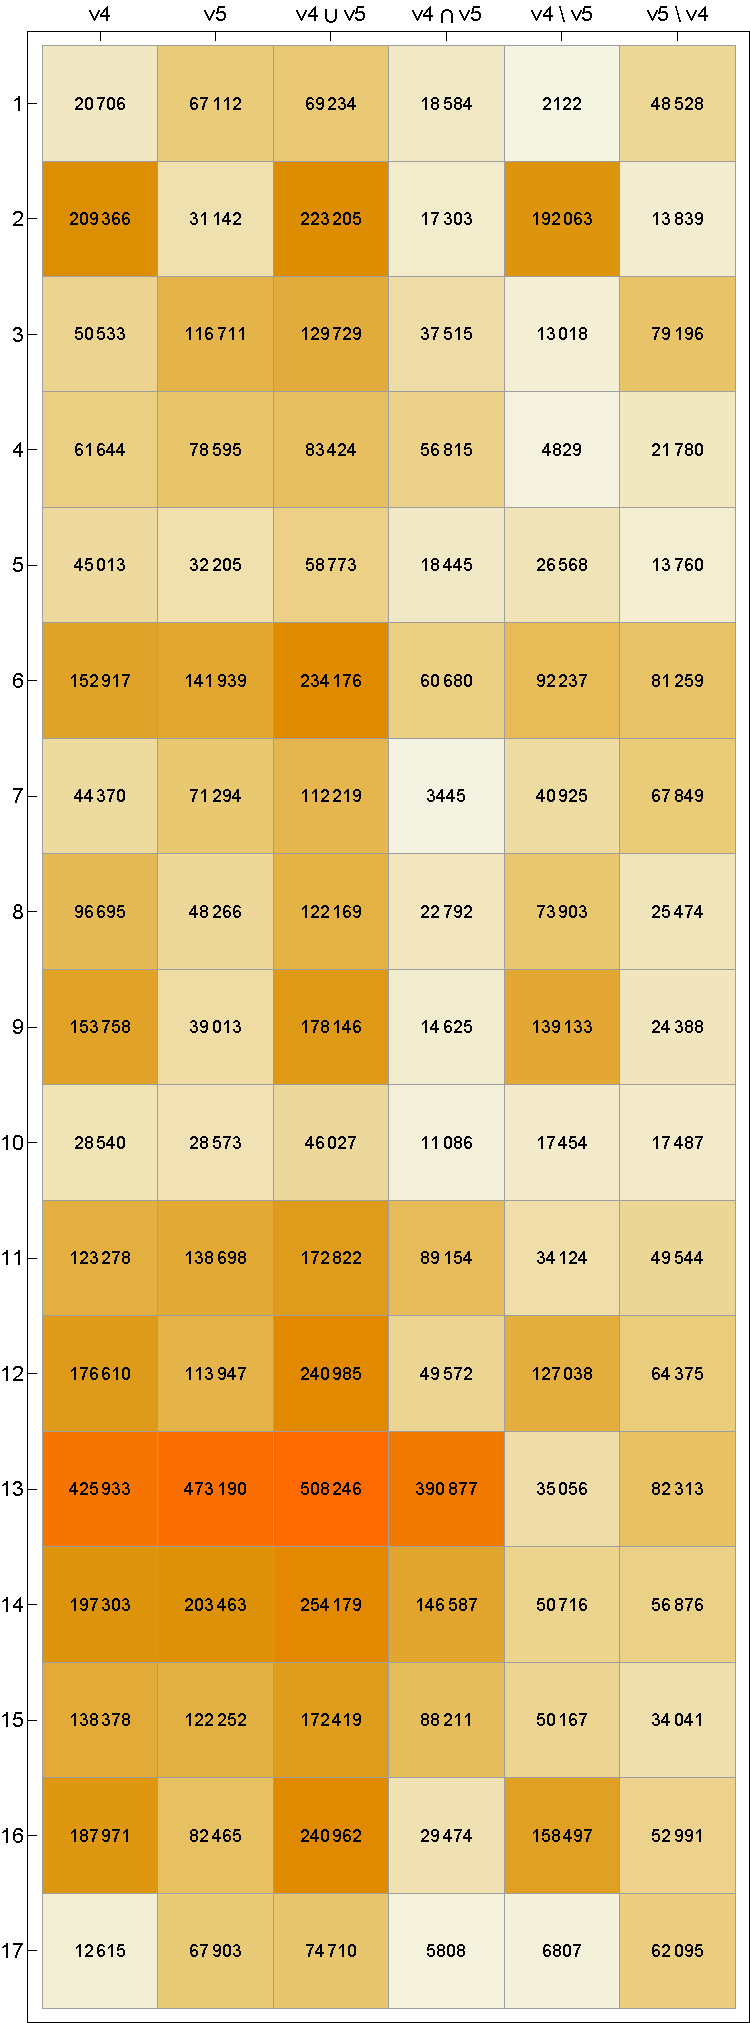
\includegraphics[width=0.5\textwidth]{figures/heatmapnumberofpublications.pdf}
%	\caption{Heatmap: Number of publications per SDG: v4, v5, v4 or v5, v4 and v5, v4 and not v5, v5 and not v4.}
%	\label{heatmapnumberofpublications}
%\end{figure}
Figures \ref{overlapv4vsv5absolute} and \ref{overlapv4vsv5relative} show the numbers as stacked bar charts in absolute and relative numbers, respectively. The results only in v4 are shown in orange, the ones only in v5 in blue and the ones in both versions in brown.
Additionally, we calculated the relative change of the cardinality from v4 to v5 and the robustness, which are defined as:
\begin{equation*}
    \text{change of cardinality} = \frac{\text{number of results from v5}-\text{number of results from v4}}{\text{number of results from v4}}\cdot100\%
\end{equation*}
and
\begin{equation*}
    \text{robustness} = \frac{\text{number of publications in v4 and v5}}{\text{number of publications in v4 or v5}}\cdot100\%
\end{equation*}
The change of cardinality gives a measure for how the number of results change from v4 to v5, the robustness a measure for the shift of the results to different publications.
\begin{figure}[H]
	\centering
  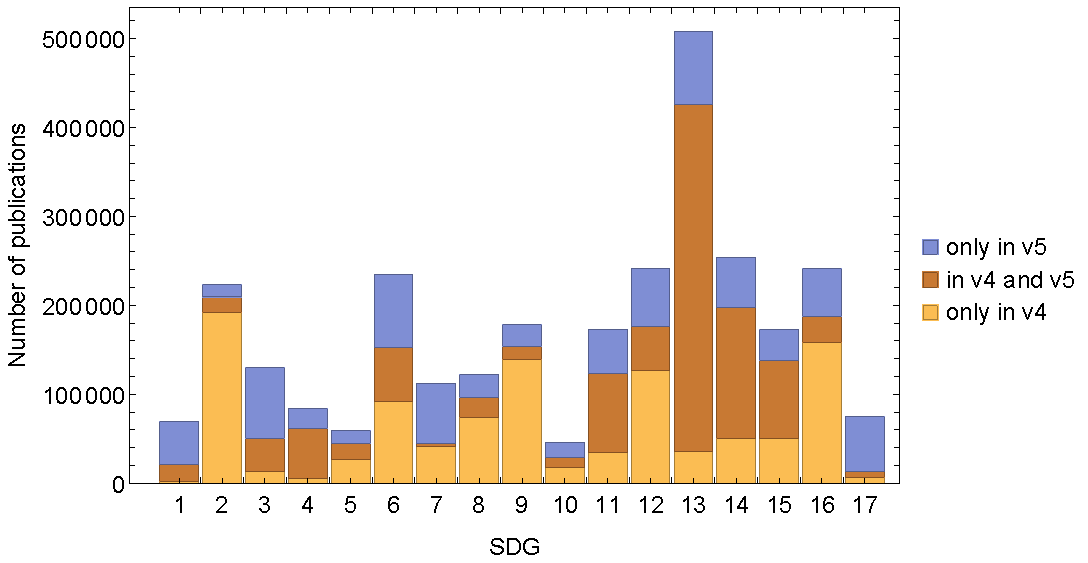
\includegraphics[width=0.75\textwidth]{figures/overlapv4vsv5barchartabsolute.pdf}
	\caption{Overlap between v4 and v5 per SDG in absolute numbers.}
	\label{overlapv4vsv5absolute}
\end{figure}
\begin{figure}[H]
	\centering
  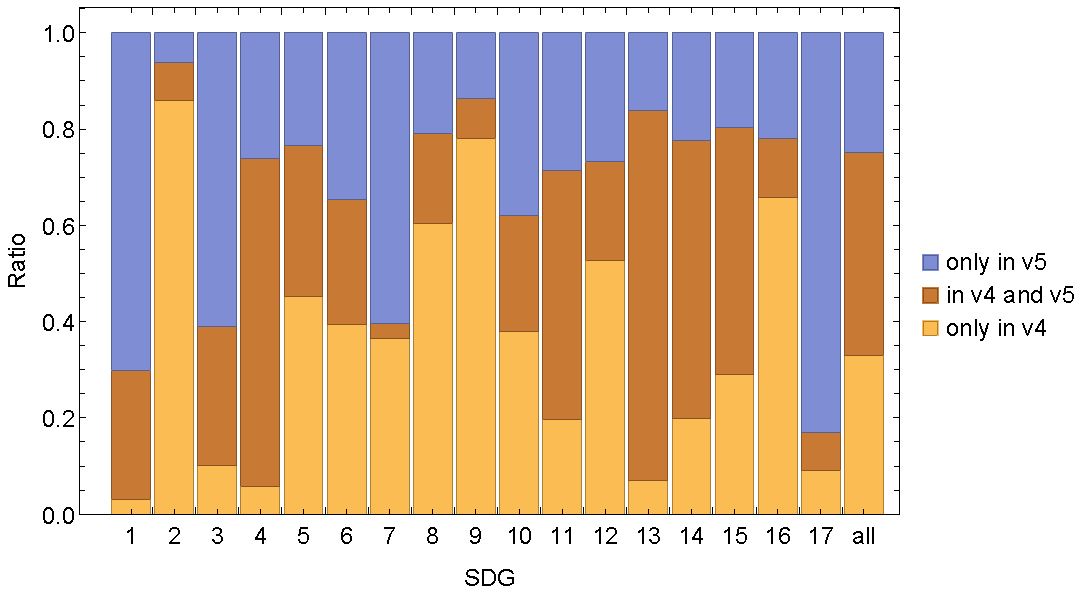
\includegraphics[width=0.75\textwidth]{figures/overlapv4vsv5barchartrelative.pdf}
	\caption{Overlap between v4 and v5 per SDG in relative numbers (normalized to the number of results in v4 OR v5 per SDG).}
	\label{overlapv4vsv5relative}
\end{figure}
We identified four SDG's where the change from v4 to v5 was very large (robustness smaller than 10\%): these are SDG02, SDG07, SDG09, and SDG17. In the next section we take a closer look at these SDG's and try to investigate the changes of the corresponding queries from a different point of view.
\begin{table}[H]
\centering 
 \begin{tabular}{ccc}
 \toprule
  SDG & change of cardinality $[\%]$  & robustness $[\%]$ \\
 \hline
 1 & 224.1 & 26.8 \\
 2 & -85.1 & 7.8 \\
 3 & 131. & 28.9 \\
 4 & 27.5 & 68.1 \\
 5 & -28.5 & 31.4 \\
 6 & -7.2 & 25.9 \\
 7 & 60.7 & 3.1 \\
 8 & -50.1 & 18.7 \\
 9 & -74.6 & 8.2 \\
 10 & 0.1 & 24.1 \\
 11 & 12.5 & 51.6 \\
 12 & -35.5 & 20.6 \\
 13 & 11.1 & 76.9 \\
 14 & 3.1 & 57.7 \\
 15 & -11.7 & 51.2 \\
 16 & -56.1 & 12.2 \\
 17 & 438.3 & 7.8 \\
 all & -10.8 & 42. \\
 \bottomrule
\end{tabular}\caption{Changes of results from v4 queries to v5 queries: relative change of the number of publications (cardinality) and shift of the results (robustness).}
\label{robustnesstable}
\end{table}


%=== WHY HOW RESULT ============================================================================

\subsection{Precision and Recall with baseline data}
\label{sec:precision-recall}
The aim in developing the new queries v5 from the v4 queries is to improve the results one gets. A way to measure this improvement can be done by looking at the precision and recall of the queries. The precision is the fraction of relevant papers among the results, the recall is the fraction of relevant papers that were found by the query.

\subsubsection{Baseline data}
 
For the calculations, we use the results from a comprehensive survey conducted among researchers based on the v4 queries \cite{vanderfeesten_survey_2020} and a basic survey among project members concerning the four SDG's with low robustness (cf. Table \ref{robustnesstable})
In the comprehensive survey, 10793 publications were checked by researchers regarding the correct classification to a specific SDG. Additionally, 4106 publications were suggested, that should be in the respective result sets.

In the basic survey among project members, for each of the SDG's with a robustness below 10\% we randomly selected 100 publications, and were checked manually regarding the correct classification.

\subsubsection{Precision}

We first calculate the precision from the basic survey for the four SDG's 02, 07, 09, and 17. The results are shown in Table \ref{precisionv5surv}.
\begin{table}[H]
\centering 
 \begin{tabular}{cccccccc}
 \toprule
 SDG & y & u & n & total & y $[\%]$ & u $[\%]$ & n $[\%]$ \\
  \hline
2 & 85 & 2 & 13 & 100 & 85.0 & 2.0 & 13.0 \\
7 & 85 & 13. & 2 & 100 & 85.0 & 13.0 & 2.0 \\
9 & 51 & 5 & 44 & 100 & 51.0 & 5.0 & 44.0 \\
17 & 63 & 13 & 24 & 100 & 63.0& 13.0 & 24.0 \\
\bottomrule
\end{tabular}
\caption{Precision of the four SDG's with the lowest robustness (v5 queries).}\label{precisionv5surv}
\end{table}
From the same data one can also calculate the precision of the v4 queries. The results are shown in Table \ref{precisionv4surv}. Note, that these results are less reliable, due to the small sample size, especially for SDG07 and SDG17. 
From the numbers in Tables \ref{precisionv5surv} and \ref{precisionv4surv} one can infer no improvement of the precision for the four SDG's with low robustness.
\begin{table}[H]
\centering 
 \begin{tabular}{cccccccc}
 \toprule
  SDG & y & u & n & total & y $[\%]$ & u $[\%]$ & n $[\%]$ \\
  \hline
2& 48 & 0 & 3 & 51 & 94.1 & 0. & 5.9 \\
7 & 7 & 0 & 0 & 7 & 100.0 & 0.0 & 0.0 \\
9 & 16 & 1 & 15 & 32 & 50.0 & 3.1 & 46.9 \\
17 & 12 & 1 & 2 & 15 & 80.0 & 6.7 & 13.3 \\
\bottomrule
\end{tabular}\caption{Precision of the four SDG's with the lowest robustness (v4 queries).}\label{precisionv4surv}
\end{table}
The precision can also be calculated based on the old comprehensive survey among researchers. More publications were classified so the results should be more valid. Additionally, there are results for the other SDG's. The results are represented in Tables  \ref{precisionv4survold} and \ref{precisionv5survold} for the v4 and v5 queries, respectively. Again, the results are more reliable for the the version of the queries, which the survey was based on. In this case we have more data for v4 as the survey was conducted with publication from the v4 queries.
\begin{table}[H]
\centering 
 \begin{tabular}{cccccc}
 \toprule
 SDG & y & n & total & y $[\%]$ & n $[\%]$ \\
 \hline
 1 & 9 & 0 & 9 & 100.00 & 0.00 \\
 2 & 186 & 414 & 600 & 31.00 & 69.00 \\
 3 & 1878 & 745 & 2623 & 71.60 & 28.40 \\
 4 & 620 & 411 & 1031 & 60.14 & 39.86 \\
 5 & 456 & 140 & 596 & 76.51 & 23.49 \\
 6 & 265 & 76 & 341 & 77.71 & 22.29 \\
 7 & 356 & 385 & 741 & 48.04 & 51.96 \\
 8 & 98 & 105 & 203 & 48.28 & 51.72 \\
 9 & 362 & 265 & 627 & 57.74 & 42.26 \\
 10 & 253 & 137 & 390 & 64.87 & 35.13 \\
 11 & 373 & 238 & 611 & 61.05 & 38.95 \\
 12 & 342 & 275 & 617 & 55.43 & 44.57 \\
 13 & 367 & 201 & 568 & 64.61 & 35.39 \\
 14 & 164 & 61 & 225 & 72.89 & 27.11 \\
 15 & 484 & 204 & 688 & 70.35 & 29.65 \\
 16 & 386 & 146 & 532 & 72.56 & 27.44 \\
 17 & 141 & 250 & 391 & 36.06 & 63.94 \\
 \bottomrule
\end{tabular}
\caption{\centering{Precision (=y[\%]) per SDG for v4 queries, based on the comprehensive survey. \\ 
v4 precision: Mean=62.8722 , Standard deviation=16.5418}}
\label{precisionv4survold}
\end{table}
\begin{table}[H]
\centering 
 \begin{tabular}{cccccc}
 \toprule
 SDG & y & n & total & y $[\%]$ & n $[\%]$ \\
 \hline
  1 & 9 & 0 & 9 & 100.00 & 0.00 \\
 2 & 33 & 19. & 52 & 63.46 & 36.54 \\
 3 & 1405 & 510 & 1915 & 73.37 & 26.63 \\
 4 & 552 & 374 & 926 & 59.61 & 40.39 \\
 5 & 208 & 60 & 268 & 77.61 & 22.39 \\
 6 & 119 & 29 & 148 & 80.41 & 19.59 \\
 7 & 60 & 15 & 75 & 80.00 & 20.00 \\
 8 & 17 & 25 & 42 & 40.48 & 59.52 \\
 9 & 41 & 17 & 58 & 70.69 & 29.31 \\
 10 & 116 & 37 & 153 & 75.82 & 24.18 \\
 11 & 279 & 159 & 438 & 63.70 & 36.30 \\
 12 & 128 & 45 & 173 & 73.99 & 26.01 \\
 13 & 347 & 183 & 530 & 65.47 & 34.53 \\
 14 & 145 & 35 & 180 & 80.56 & 19.44 \\
 15 & 294 & 137 & 431 & 68.21 & 31.79 \\
 16 & 65 & 22 & 87 & 74.71 & 25.29 \\
 17 & 71 & 95 & 166 & 42.77 & 57.23 \\
 \bottomrule
\end{tabular}
\caption{\centering{Precision (=y[\%]) per SDG for v5 queries, based on the comprehensive survey. \\ 
v5 precision: Mean=70.0502 , Standard deviation=14.1167}}
\label{precisionv5survold}
\end{table}
The differences of the precision scores can be inferred from the bar chart in Figure \ref{precisionbarchart}. For 13 out of the 17 SDGs there is an (minor) improvement of the precision, 3 SDGs show an (minor) decrease, for one SDG it does not change. One should keep in mind that at this point the data for the v5 queries is rather limited.
We find lowest precision scores from the results of v5 queries for SDG 9 (51\%, based on the basic survey) and SDG 8 (40\%, based on the comprehensive survey). We find mayor improvements of the precision for SDGs 2 and 7 (from 31\% to 61\% and from 48\% to 80\%, respectively); on average, the precision increased from 63\% to 70\%.
\begin{figure}[H]
	\centering
  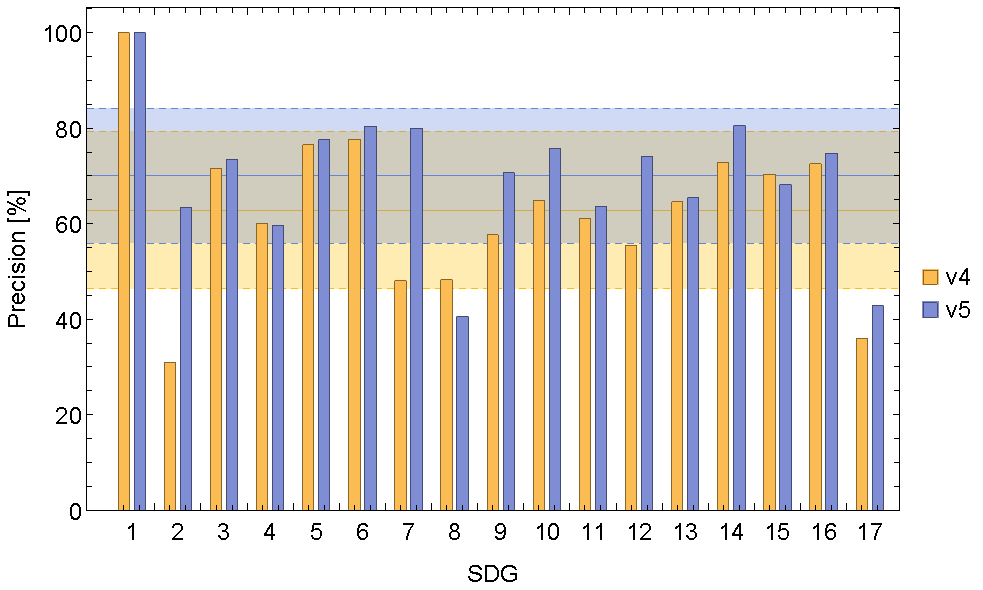
\includegraphics[width=0.75\textwidth]{figures/precisionbarchart.pdf}
	\caption{\centering{ Precision v4 vs v5, based on the comprehensive survey among researchers \\
	v4: mean=62.8722 standard deviation=16.5418 \\ v5: mean=70.0502 standard deviation=14.1167}
}
	\label{precisionbarchart}
\end{figure}

\subsubsection{Recall}

The recall of the two versions of the query can be calculated from the publications suggested by the researchers in the comprehensive survey. The numbers can be found in Table \ref{recalltable}. Overall, 4106 publications were suggested, the distribution of these suggestions is very skew and ranges from 5 for SDG 1 to 1255 for SDG 3.
\begin{table}[H]
\centering 
 \begin{tabular}{cccccc}
 \toprule
  SDG & suggested publications & v4 & v5 & v4 $[\%]$ & v5 $[\%]$ \\
  \hline
 1 & 5 & 0 & 1 & 0.00 & 20.00 \\
 2 & 89 & 30 & 22 & 33.71 & 24.72 \\
 3 & 1255 & 9 & 23 & 0.72 & 1.83 \\
 4 & 127 & 8 & 17 & 6.30 & 13.39 \\
 5 & 493 & 76 & 37 & 15.42 & 7.51 \\
 6 & 543 & 11 & 12 & 2.03 & 2.21 \\
 7 & 373 & 20 & 14 & 5.36 & 3.75 \\
 8 & 83 & 6 & 6 & 7.23 & 7.23 \\
 9 & 246 & 20 & 12 & 8.13 & 4.88 \\
 10 & 73 & 2 & 3 & 2.74 & 4.11 \\
 11 & 121 & 12 & 15 & 9.92 & 12.40 \\
 12 & 132 & 24 & 22 & 18.18 & 16.67 \\
 13 & 94 & 50 & 55 & 53.19 & 58.51 \\
 14 & 57 & 25 & 23 & 43.86 & 40.35 \\
 15 & 282 & 28 & 31 & 9.93 & 10.99 \\
 16 & 80 & 18 & 5 & 22.50 & 6.25 \\
 17 & 53 & 5 & 7 & 9.43 & 13.21 \\
 all & 4106 & 344 & 305 & 8.38 & 7.43 \\
 \bottomrule
\end{tabular}
\caption{\centering{Recall per SDG, based on the comprehensive survey.\\
v4 recall: Mean=14.6, Standard deviation = 15.4 \\
v5 recall: Mean=14.6, Standard deviation = 14.9}
}
\label{recalltable}
\end{table}




\begin{figure}[H]
	\centering
  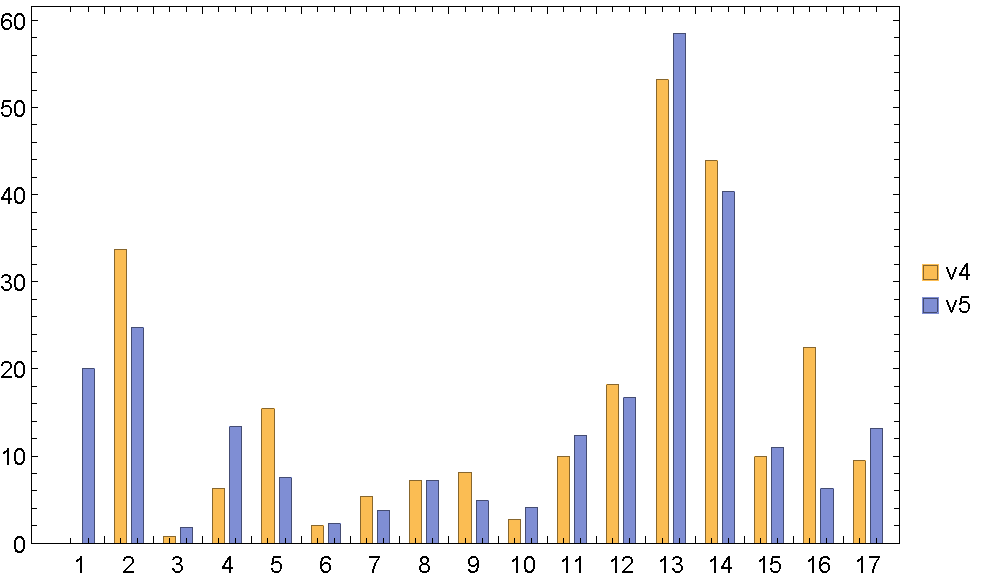
\includegraphics[width=0.75\textwidth]{figures/recallbarchart.pdf}
	\caption{Recall v4 vs v5}
	\label{recallbarchart}
\end{figure}

\begin{figure}[H]
    \centering
         \begin{subfigure}{0.49\textwidth}
                     \centering
            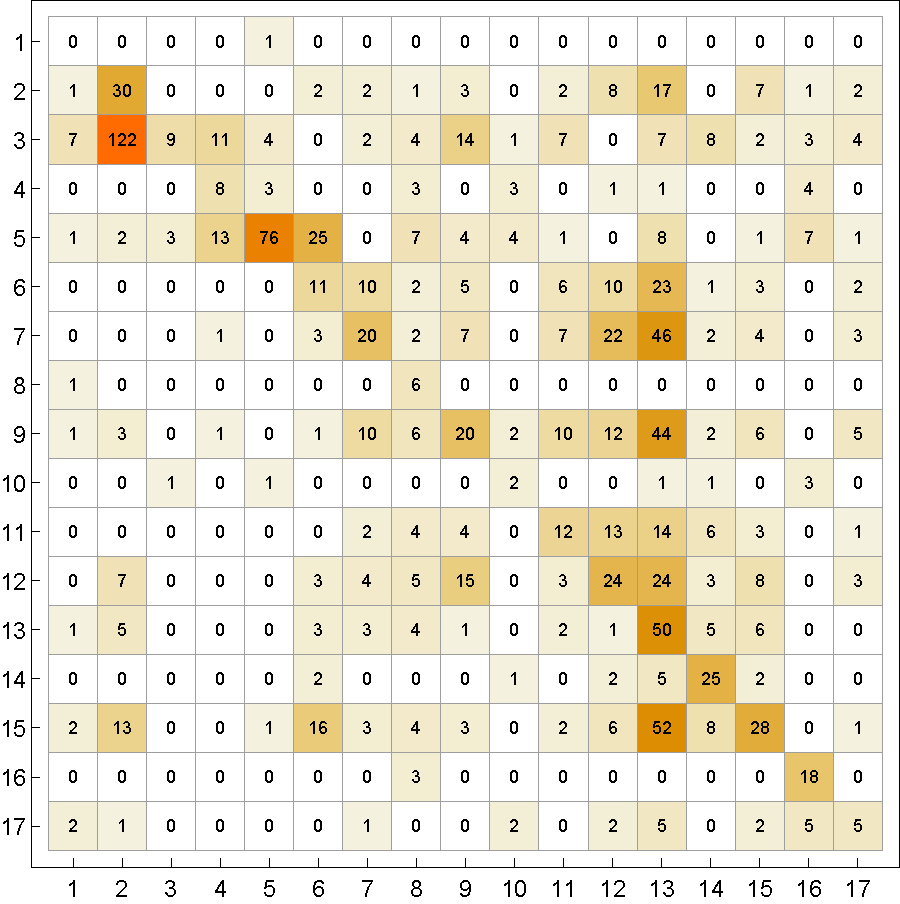
\includegraphics[width=\textwidth]{figures/recallmatrixv4.pdf}
            \caption{v4}
            \label{subfig1}
        \end{subfigure}
             \hfill
         \begin{subfigure}{0.49\textwidth}
                     \centering
            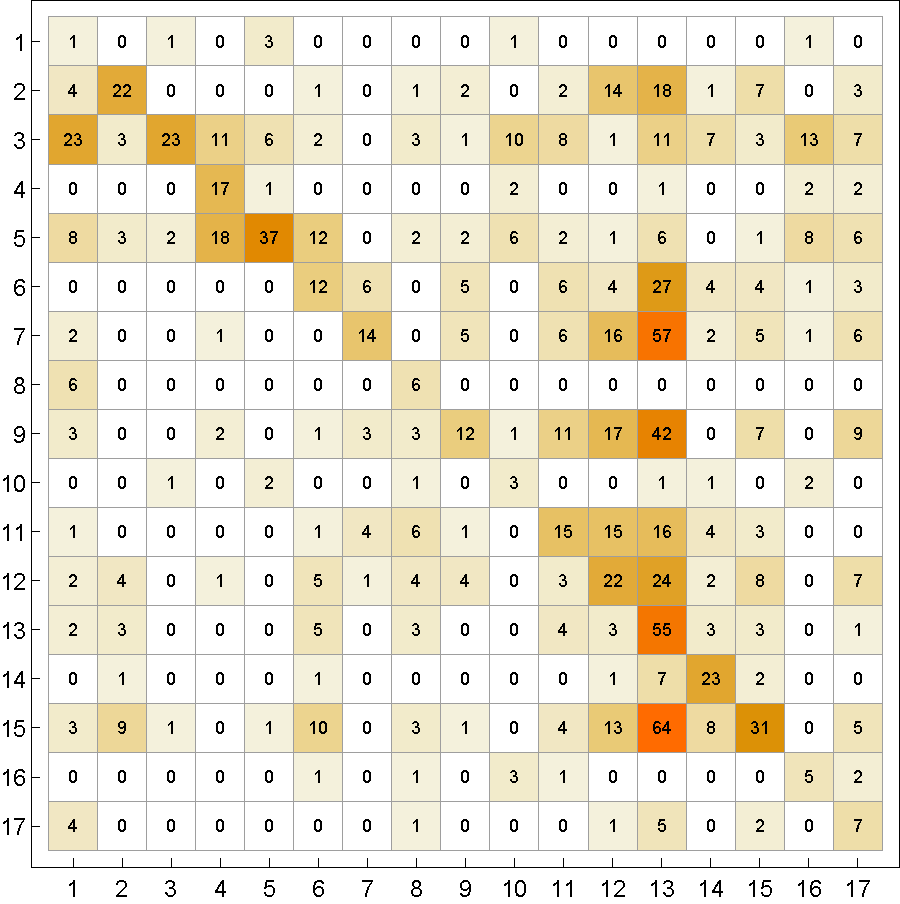
\includegraphics[width=\textwidth]{figures/recallmatrixv5.pdf}
            \caption{v5}
            \label{subfig2}
        \end{subfigure}
        \caption{Recall data for v4 and v5 queries:}
\end{figure}


\subsubsection{Accuracy: Combining Precision and Recall}
In this section we combine the outcomes of the precision and recall, which gives a measure of the accuracy of the different queries for each of the SDG's. We use the F-score to calculate the accuracy:

\begin{equation*}
    F_1 = \frac{\text{precision}\cdot\text{recall}}{\text{precision}+\text{recall}}
\end{equation*}

This results in the following results:

\begin{table}[H]
\centering 
\begin{tabular}{c c ccc c ccc}
\toprule
&&\multicolumn{3}{c}{v4}&&\multicolumn{3}{c}{v5}\\
\cline{3-5} \cline{7-9}
SDG && precision & recall & F score && precision & recall & F score \\
 \hline
 1 && 0.00 & 100.00 & 0.00 && 20.00 & 100.00 & 33.33 \\
 2 && 33.71 & 31.00 & 32.30 && 24.72 & 63.46 & 35.58 \\
 3 && 0.72 & 71.60 & 1.42 && 1.83 & 73.37 & 3.58 \\
 4 && 6.30 & 60.14 & 11.40 && 13.39 & 59.61 & 21.86 \\
 5 && 15.42 & 76.51 & 25.66 && 7.51 & 77.61 & 13.69 \\
 6 && 2.03 & 77.71 & 3.95 && 2.21 & 80.41 & 4.30 \\
 7 && 5.36 & 48.04 & 9.65 && 3.75 & 80.00 & 7.17 \\
 8 && 7.23 & 48.28 & 12.57 && 7.23 & 40.48 & 12.27 \\
 9 && 8.13 & 57.74 & 14.25 && 4.88 & 70.69 & 9.13 \\
 10 && 2.74 & 64.87 & 5.26 && 4.11 & 75.82 & 7.80 \\
 11 && 9.92 & 61.05 & 17.06 && 12.40 & 63.70 & 20.75 \\
 12 && 18.18 & 55.43 & 27.38 && 16.67 & 73.99 & 27.21 \\
 13 && 53.19 & 64.61 & 58.35 && 58.51 & 65.47 & 61.80 \\
 14 && 43.86 & 72.89 & 54.77 && 40.35 & 80.56 & 53.77 \\
 15 && 9.93 & 70.35 & 17.40 && 10.99 & 68.21 & 18.93 \\
 16 && 22.50 & 72.56 & 34.35 && 6.25 & 74.71 & 11.54 \\
 17 && 9.43 & 36.06 & 14.96 && 13.21 & 42.77 & 20.18 \\
 \bottomrule
\end{tabular}
\caption{Precision, recall and F score for v4 and v5 queries.}
\label{precisiondatatab}
\end{table}

Figure \ref{f1barchart} shows the F scores of the SDG queries of the different versions side-by-side. 
\begin{figure}[H]
	\centering
  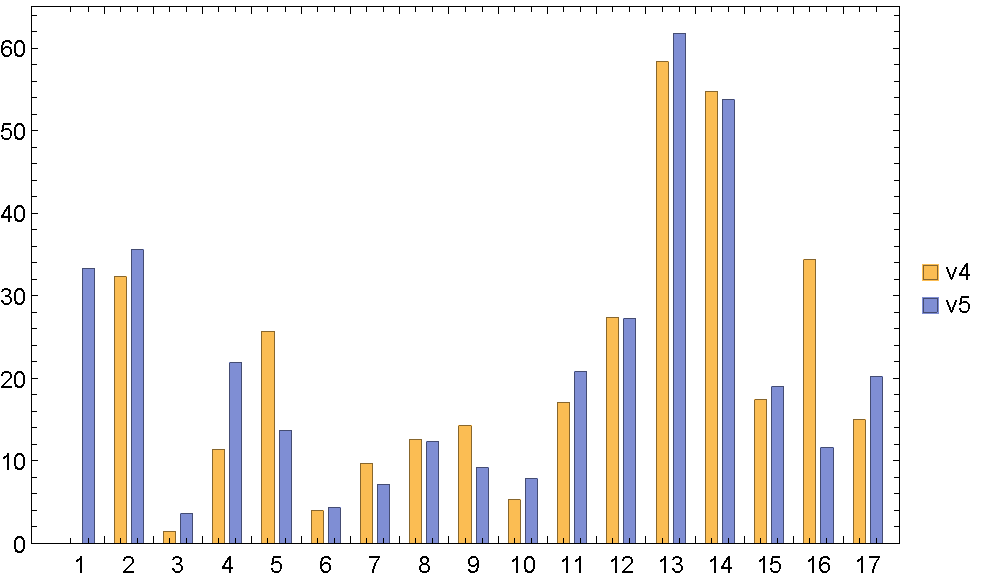
\includegraphics[width=0.75\textwidth]{figures/f1barchart.pdf}
	\caption{F score v4 vs v5}
	\label{f1barchart}
\end{figure}

Here see that for SDG's 1, 2, 13, 14 and 16 have higher F scores compared to the other SDG's. We also see that some SDG's F scores increased and decreased from version 4 to version 5.

We want to know how or if that increase or decrease is related to the amount of change of the publications of the result sets of each SDG. We combined the change of F score between v4 and v5 from table \ref{precisiondatatab} with the robustness score of table \ref{robustnesstable}, resulting in the following chart. 

\begin{figure}[H]
	\centering
  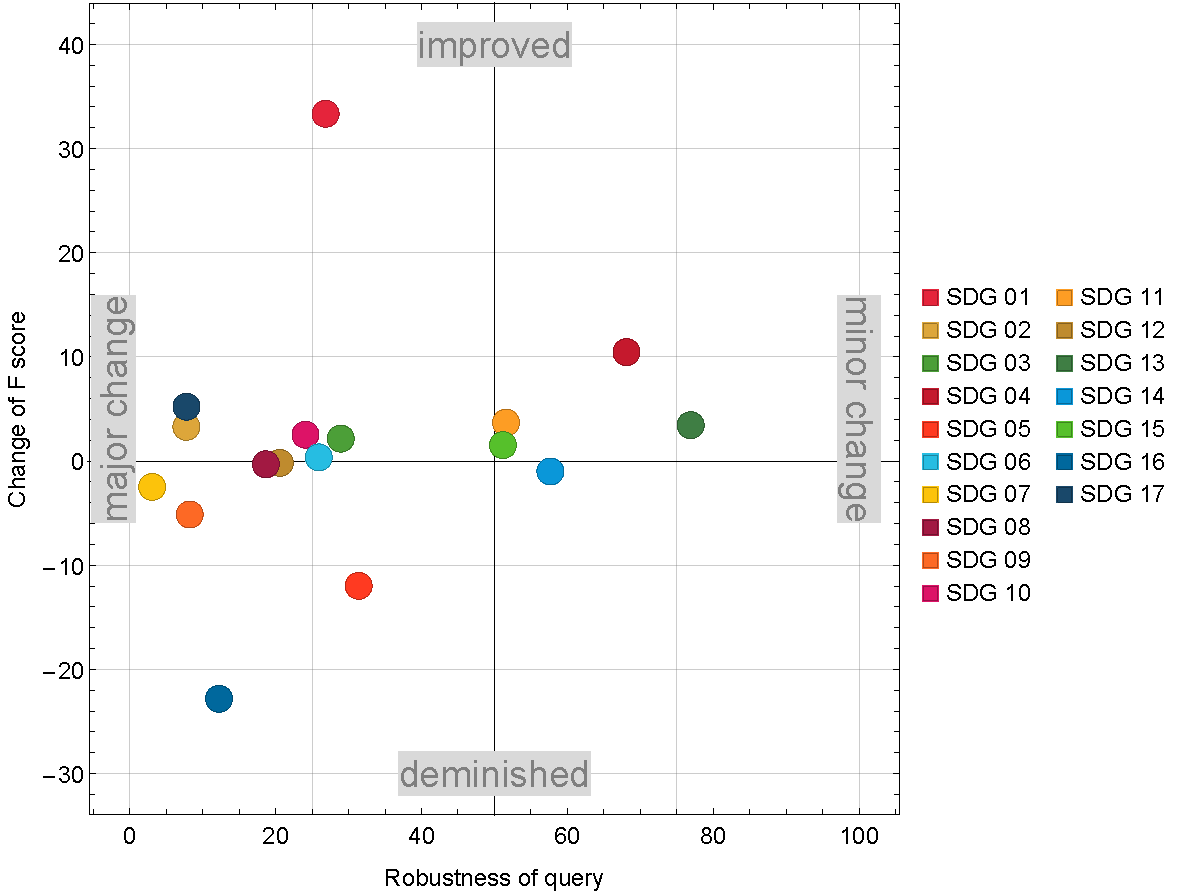
\includegraphics[width=\textwidth]{figures/scatterplot1-fscore-robustness.pdf}
	\caption{f score change vs robustness of SDG's}
	\label{fscore-vs-robustnes}
\end{figure}

We see in figure \ref{fscore-vs-robustnes} how the SDG's have improved or diminished in F score in SDG queries version 5, and whether that required a small or big change of the publications in the SDG result sets to sort for that effect.

F-scores don't distinguish between precision and recall. To show if the accuracy it based on precision or the recall, we make for each version v4 and v5 a bubble plot, where we plot the precision, recall and the tested sample sizes for each of the SDG. 

% Make two bubble plots, v4 and v5, with precision (y-axis) recall (x-axis), sample sizes (bubble size) for each SDG.


\begin{figure}[H]
	\centering
  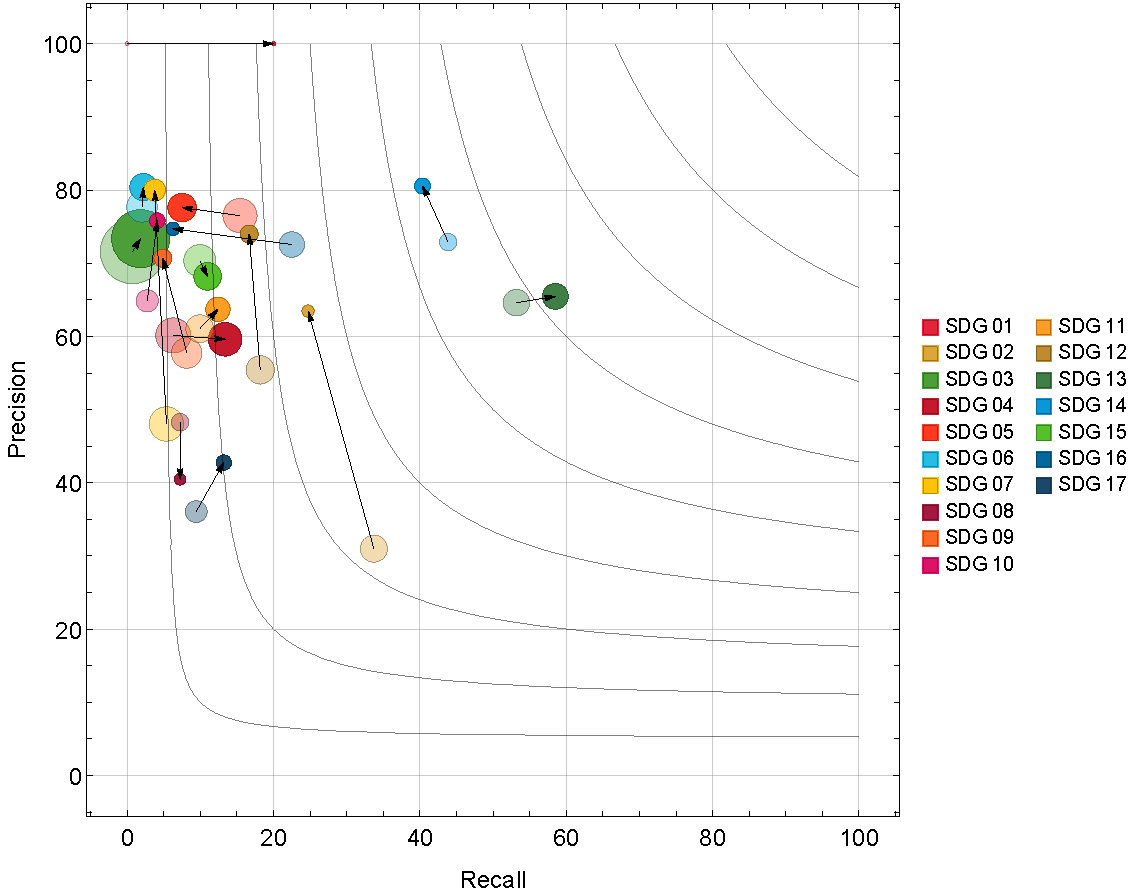
\includegraphics[width=\textwidth]{figures/bubblechart2.pdf}
	\caption{Precision, recall and amount of publications suggested and selected by expert researchers for v4 and v5 queries. V4 SDG's in semi-transparent color, v5 SDG's in full colors. The iso-lines show the constant F-scores from 5 (bottom left) to 45 (top right). }
	\label{bubblechart}
\end{figure}

Here we see that our queries mainly moved to increase the precision, without big changes in the F scores, at the cost of a low recall. 

This means \emph{the Aurora SDG queries version 5 collect a small number of papers, but the papers collected are in the majority of the cases relevant publications related to the SDG Goals and Targets.}

\section{Discussion \& Conclusions}
What conclusions can we draw the what we know , looking at the results. Are the questions answered?

Having a labeled corpus aiming at precision of the labeling of the SDG goals, allows us to use the queries to generate a labeled corpus that can be used in Machine learning. \cite{zhang_matching_2020}  To gain recall, we can feed the machine learning phase with a language model to label papers to an SDG that is closely related to similar semantic concepts. This is something we are unable to accomplish with boolean queries, due to the binary nature of a keyword search. This result gives confidence we have a solid foundation to build a machine learning model from the labeled corpus with the Aurora SDG queries version 5. 

With IDfuse \footnote{IDfuse is a Dutch startup that uses machine learning to improve grant proposal writing. \url{https://idfuse.nl/} } we did some early experimentation on enhancing the results of the query based model with machine learning using the widely used BERT model, retrained for Scientific content (SciBERT)\footnote{\url{https://github.com/allenai/scibert}}. 
To train the SciBert model to label publications to the SDG's, IDfuse loaded the OpenAIRE Resaerch Graph in to ElasticSearch, translated\footnote{Scopus to Elastic Search Translator: \url{https://github.com/martijnvanbeers/booque} for creating training corpus with OpenAIRE Research Graph} the Aurora queries version 5 from a Scopus Query Language to the ElasticSearch Query Language, and used the result sets to train the model.

\begin{figure}[H]
	\centering
  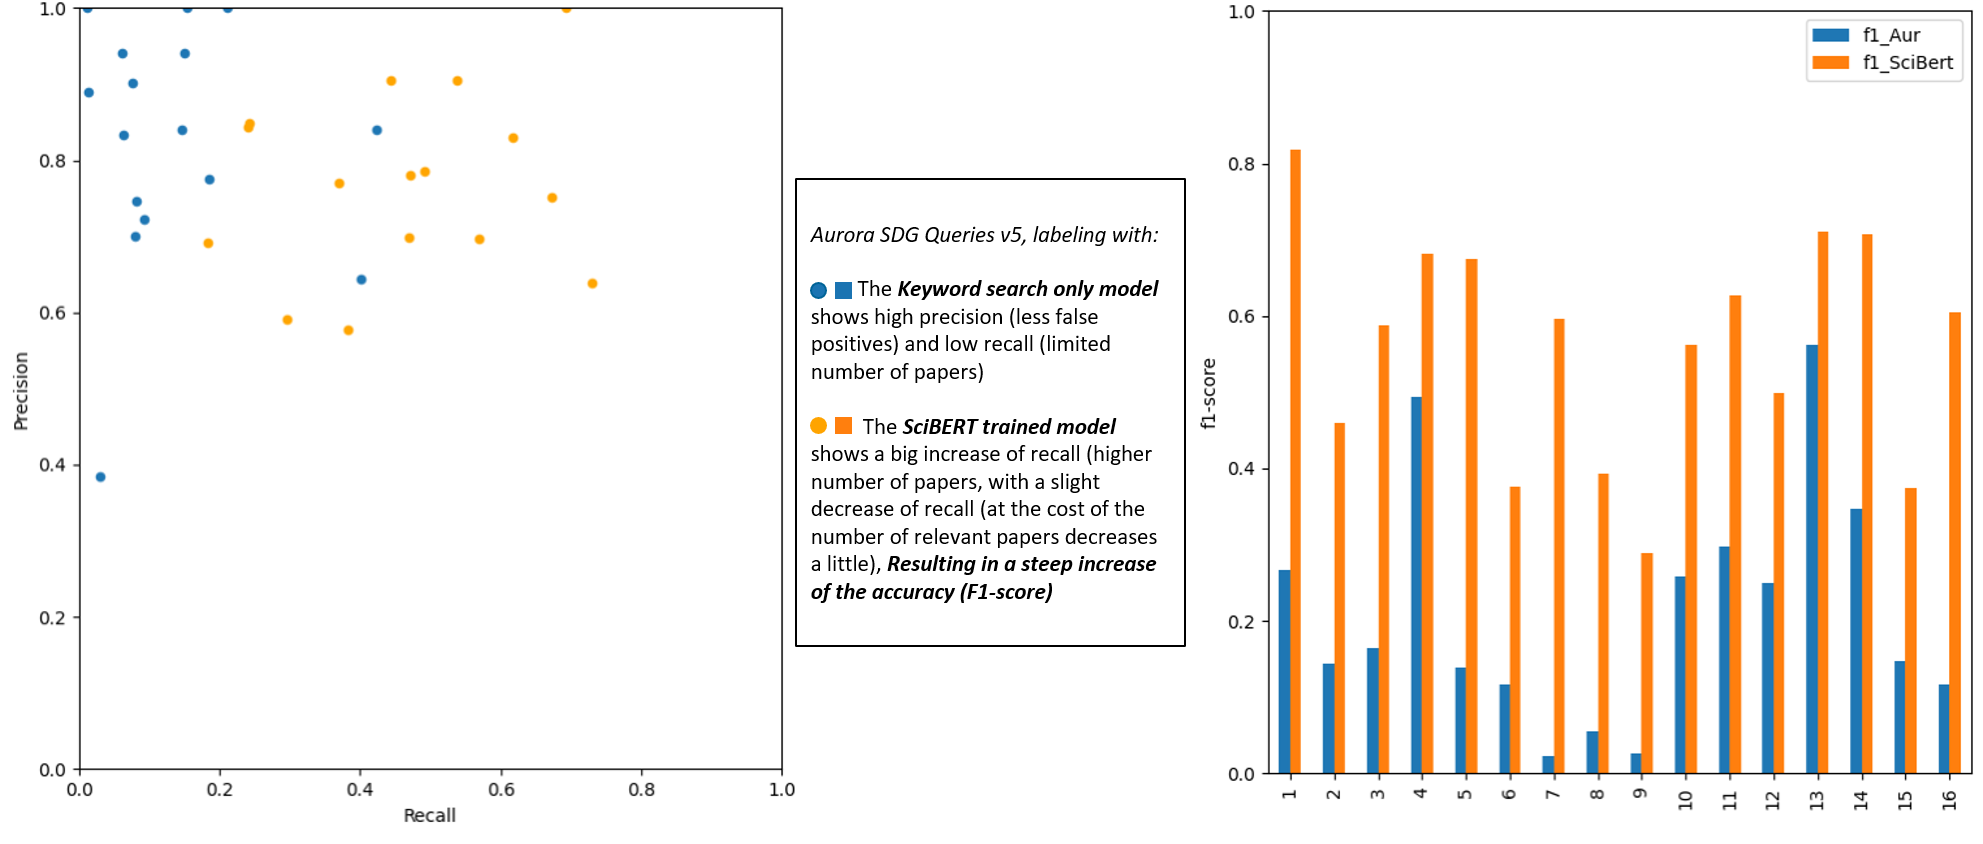
\includegraphics[width=\textwidth]{figures/BERTmodel-improves-recall.png}
	\caption{Training label sets with SciBERT language model improves the recall of the Boolean queries, at a cost of slight decrease of precision.}
	\label{BERTmodel}
\end{figure}

In figure \ref{BERTmodel} we see that the Keyword-search-only model (blue dots and bars) shows high precision (less false positives) and low recall (limited number of papers). The SciBERT-trained model (yellow/orange dots and bars) shows on the left chart a big increase of recall, with a slight decrease of recall at a slight cost of precision, resulting on the right chart in a steep increase of the accuracy (F1-score).

This early experiment gives us confidence we can use such advanced language models to classify the SDG's, while increasing the number of research papers to be included in the result set for the SDG's, and that this larger result set will contain papers that are still relevant to the labeled SDG's.

Increasing recall, without sacrificing much of the precision was our first goal to include research in the SDG's we could not capture using Boolean queries. The next step is if we can capture also research written in other languages than English to the SDG's. Fortunately BERT language models are capable of cross-language classifications while being trained in only one language. This is something we need to investigate further.


\bibliographystyle{unsrt}  
\bibliography{references}

\end{document}
